\documentclass[conference]{IEEEtran}

\usepackage{cite}


\ifCLASSINFOpdf
  \usepackage[pdftex]{graphicx}

  \graphicspath{{../pdf/}{../jpeg/}}

  \DeclareGraphicsExtensions{.pdf,.jpeg,.png}
\else

\fi

\usepackage{caption}
\usepackage{subcaption}

\usepackage{amsmath}
\usepackage{multirow}
\usepackage{multicol}

\usepackage{algorithmic}

\usepackage{array}
\usepackage{color}

\hyphenation{op-tical net-works semi-conduc-tor}


\begin{document}

\title{\color{blue} On-Chip \color{black} Output Stage Design for  \color{blue} A \color{black} Continuous Class F Power Amplifier}

\author{\IEEEauthorblockN{Anil Kumar Kumaran\IEEEauthorrefmark{1},
M. D'Avino\IEEEauthorrefmark{2},
\color{blue} Leo C.N. de Vreede\IEEEauthorrefmark{1}, and 
Morteza S. Alavi \color{black} \IEEEauthorrefmark{1}} 
\IEEEauthorblockA{\IEEEauthorrefmark{1} Electronic Circuits and Architecture (ELCA) Research Group, Delft University of Technology \\
	\IEEEauthorblockA{\IEEEauthorrefmark{2} Catena B.V., Delft, The Netherlands} \\Email: a.k.kumaran@tudelft.nl}}

\maketitle

\begin{abstract}
Continuous Class F (CCF) power amplifiers (PAs) overcome Class F PA's disadvantage of narrow bandwidth by eliminating \color{blue} short-circuit requirements at the $2^{nd}$ harmonic. \color{black} At the same time, CCF maintains \color{blue} a \color{black} peak efficiency of \textit{90.7\%}\color{blue}, \color{black} which is higher than the traditional Class A and \color{blue} B \color{black} peak efficiency. This paper explains the equations governing the CCF mode of operation and then illustrates the step by step procedure to design \color{blue} four \color{black} different output networks for CCF using lossless lumped components for \color{blue} a \textit{2.1--2.7 GHz} band. \color{black}
The design comprising \color{blue} a \color{black} second harmonic trap and no RF choke is chosen \color{blue} due to presenting \color{black} a flatter real part \color{blue} impedance \color{black} \color{blue} along with \color{black} a smaller reactive part at the $1^{st}$ harmonic\color{blue}, and \color{black} the least number of \color{blue} on-chip \color{black} lumped components.
\end{abstract}

\vspace{1mm}
% keywords
\begin{IEEEkeywords}
Continuous class F \color{blue} (CFF) \color{black} , Output matching network, Power amplifier \color{blue} (PA) \color{black} , Harmonic termination, Differential mode analysis, Common mode analysis. 
\end{IEEEkeywords}



\ifCLASSOPTIONpeerreview
\begin{center} \bfseries EDICS Category: 3-BBND \end{center}
\fi

\IEEEpeerreviewmaketitle

\section{Introduction}
\color{blue} Today, \color{black} there is an increased demand for high-speed \color{blue} and low-cost transmissions in 4/5G and wireless connectivity \color{black} networks. \color{blue} A CMOS-based transmitter (TX) is a viable architecture to address these requirements as it facilitates the implementation of System-on-Chip (SoC) solution at a low cost. However, the TX power amplifier (PA) is the most challenging blocks \color{black}  in making CMOS SoC, because \color{blue} it should offer \color{black} high-efficiency \color{blue} while meeting the stringent spectral mask  and in-band linearity requirements of wireless systems \color{black} even at backed-off power levels. Currently, \color{blue} most of TX architectures employ linear class A/B PAs. Nevertheless, their ideal \color{black} peak efficiencies are only \color{blue}\textit{50}/\textit{78\%} \color{black} respectively, due to \color{blue} a \color{black} large overlap between the drain voltage\color{blue}/\color{black}current \color{blue}  waveforms (Fig.\ref{fig:CA_wave_VI}-\ref{fig:CB_wave_VI}). \color{black}

\color{blue}On the other hand, class  F \color{black} PAs \color{blue} ideally \color{black} achieve peak efficiency of 100\% by utilizing harmonic-frequency resonators to make short-circuit at even harmonics and open-circuit at odd harmonics to engineer the drain voltage and current with no overlap (refer Figure \ref{fig:ICF_wave_VI}). But in reality, controlling all the harmonics doesn't provide much increase in peak efficiency. On the other hand, it increases the complexity of circuit and component losses which in turn reduces efficiency. Therefore, practical implementation of class F use up to $3^{rd}$ harmonic in the voltage waveform and achieves peak efficiency of \textit{90.7\%} due to increase in overlap region compared to ideal class F (shown in Figure \ref{fig:CF_wave_VI}) \cite{Raab_max_eff}.
\begin{figure}[h]
\centering
\captionsetup{font=footnotesize}
\begin{subfigure}{0.24\textwidth}
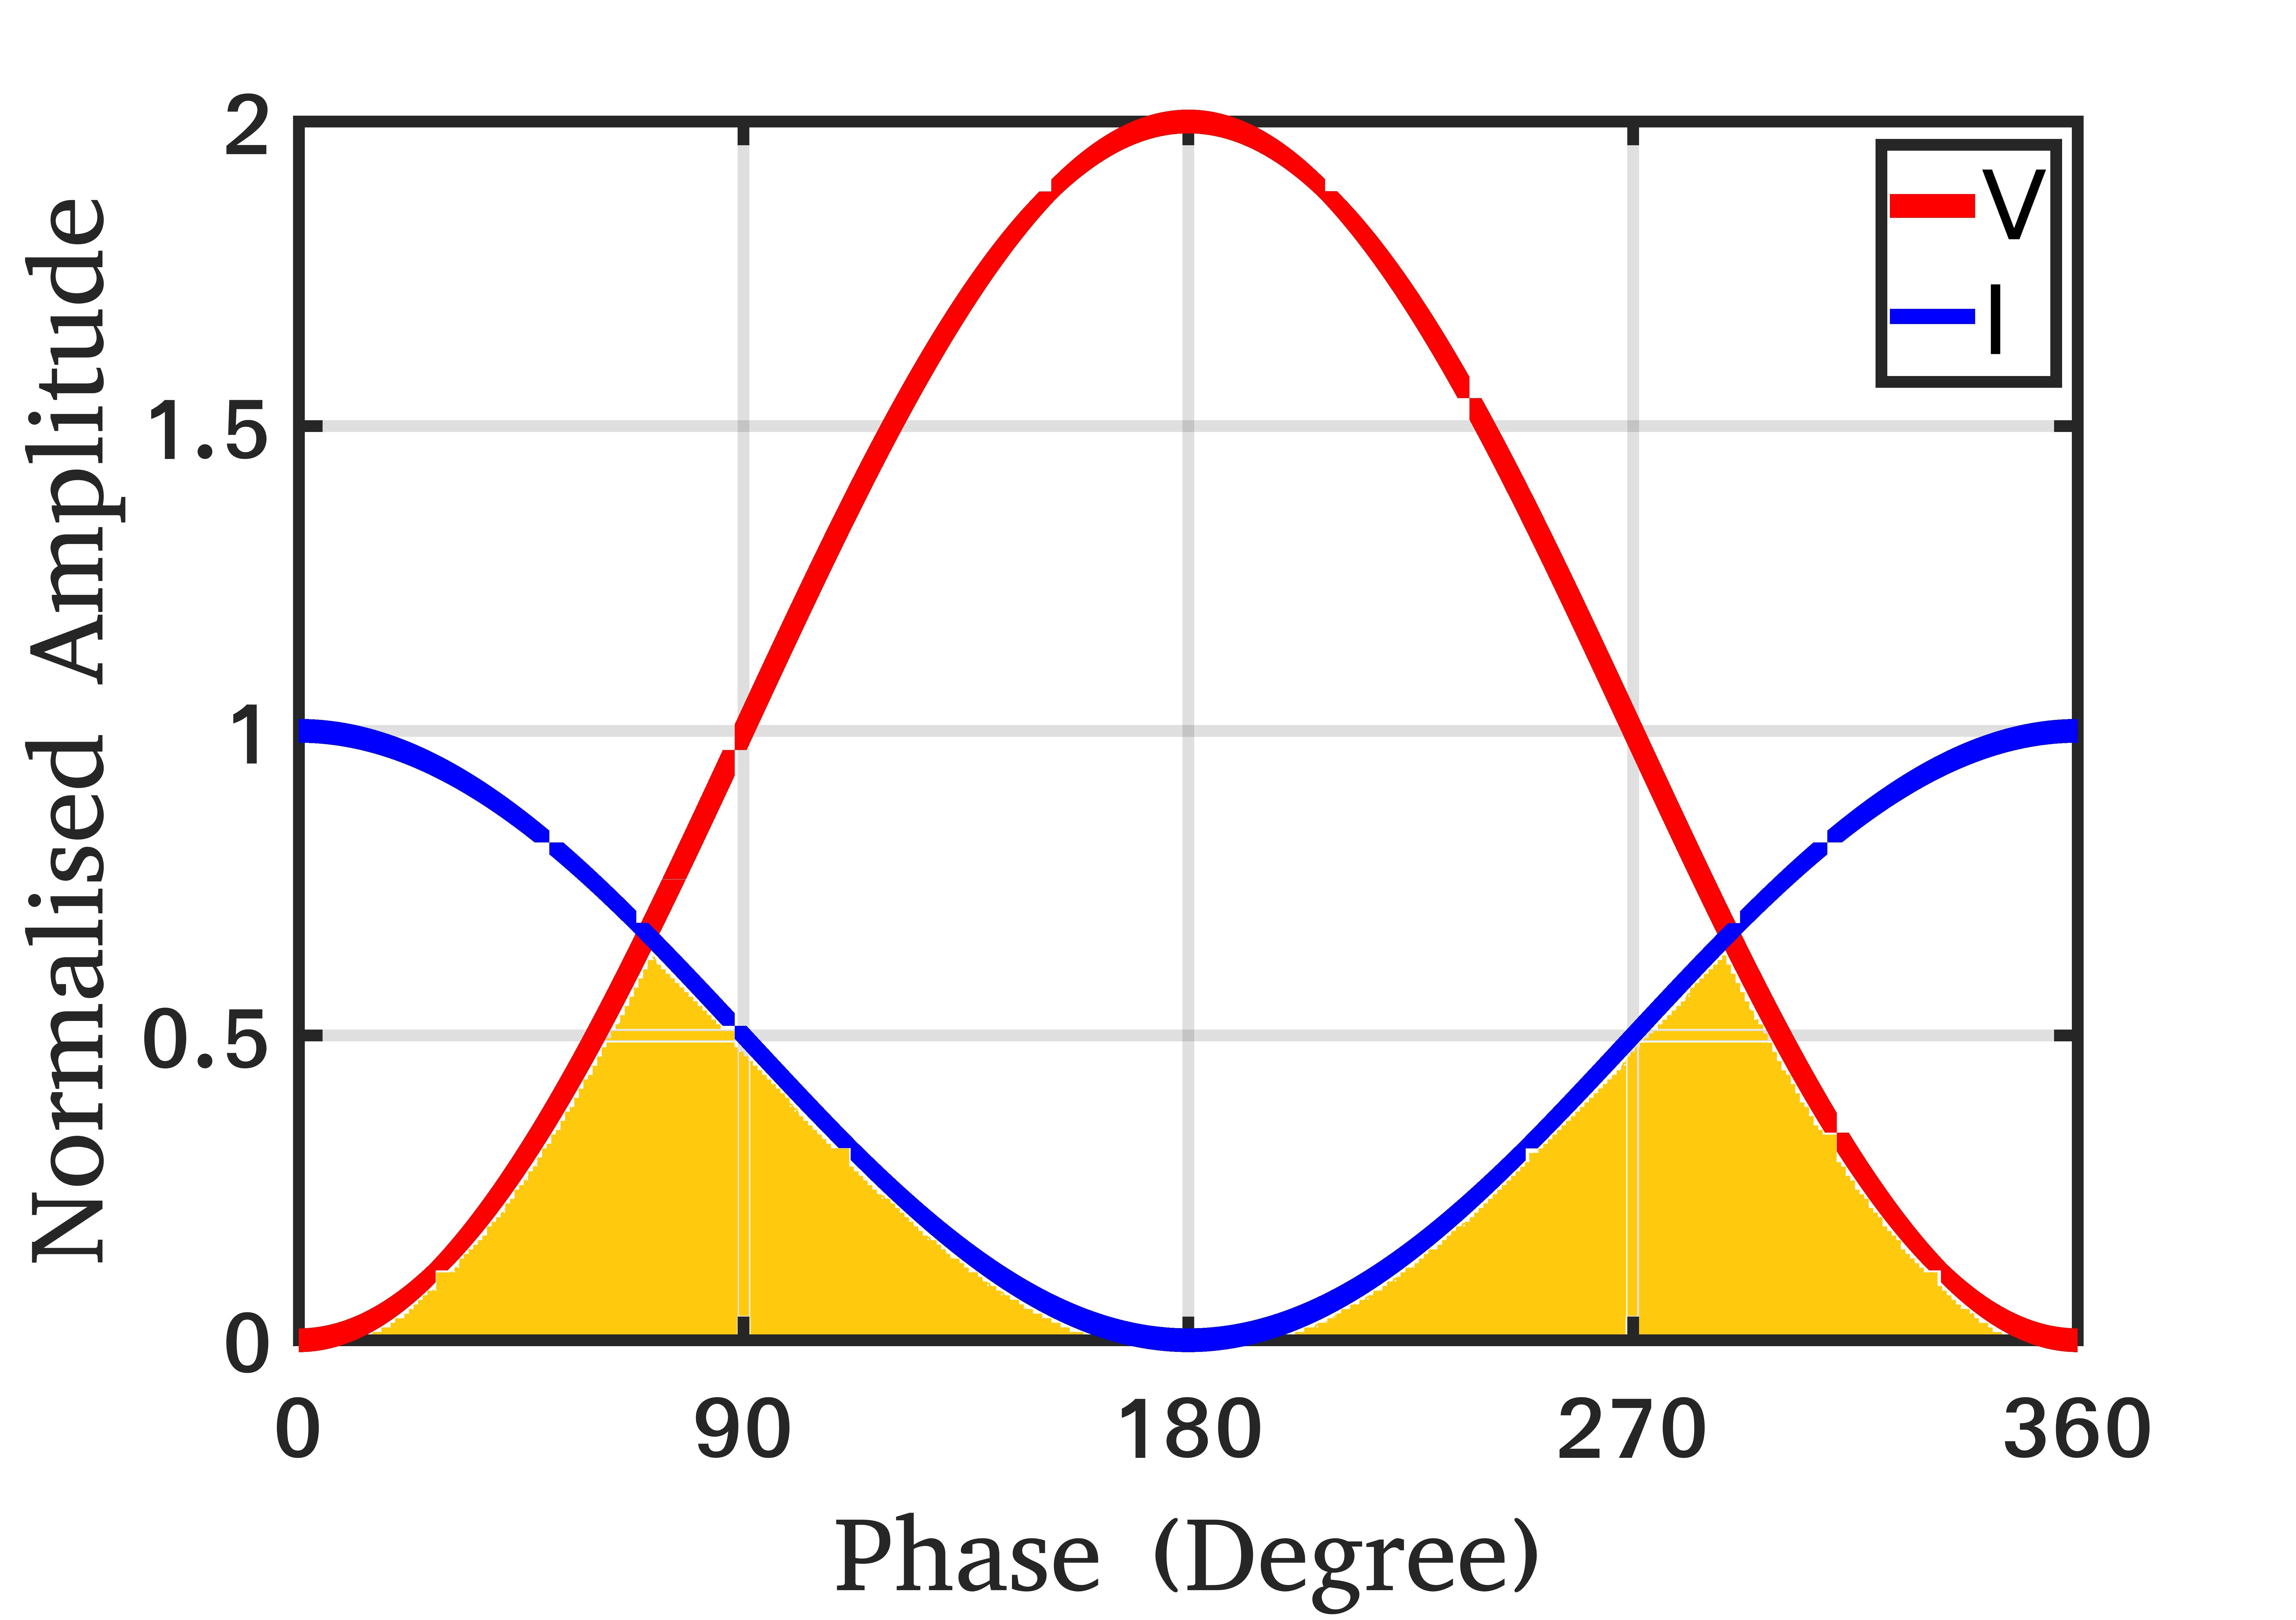
\includegraphics[width=0.9\textwidth]{Images/Intro/ClassA_shaded.jpg}
\caption{Class A}
\label{fig:CA_wave_VI}
\end{subfigure}
\begin{subfigure}{0.24\textwidth}
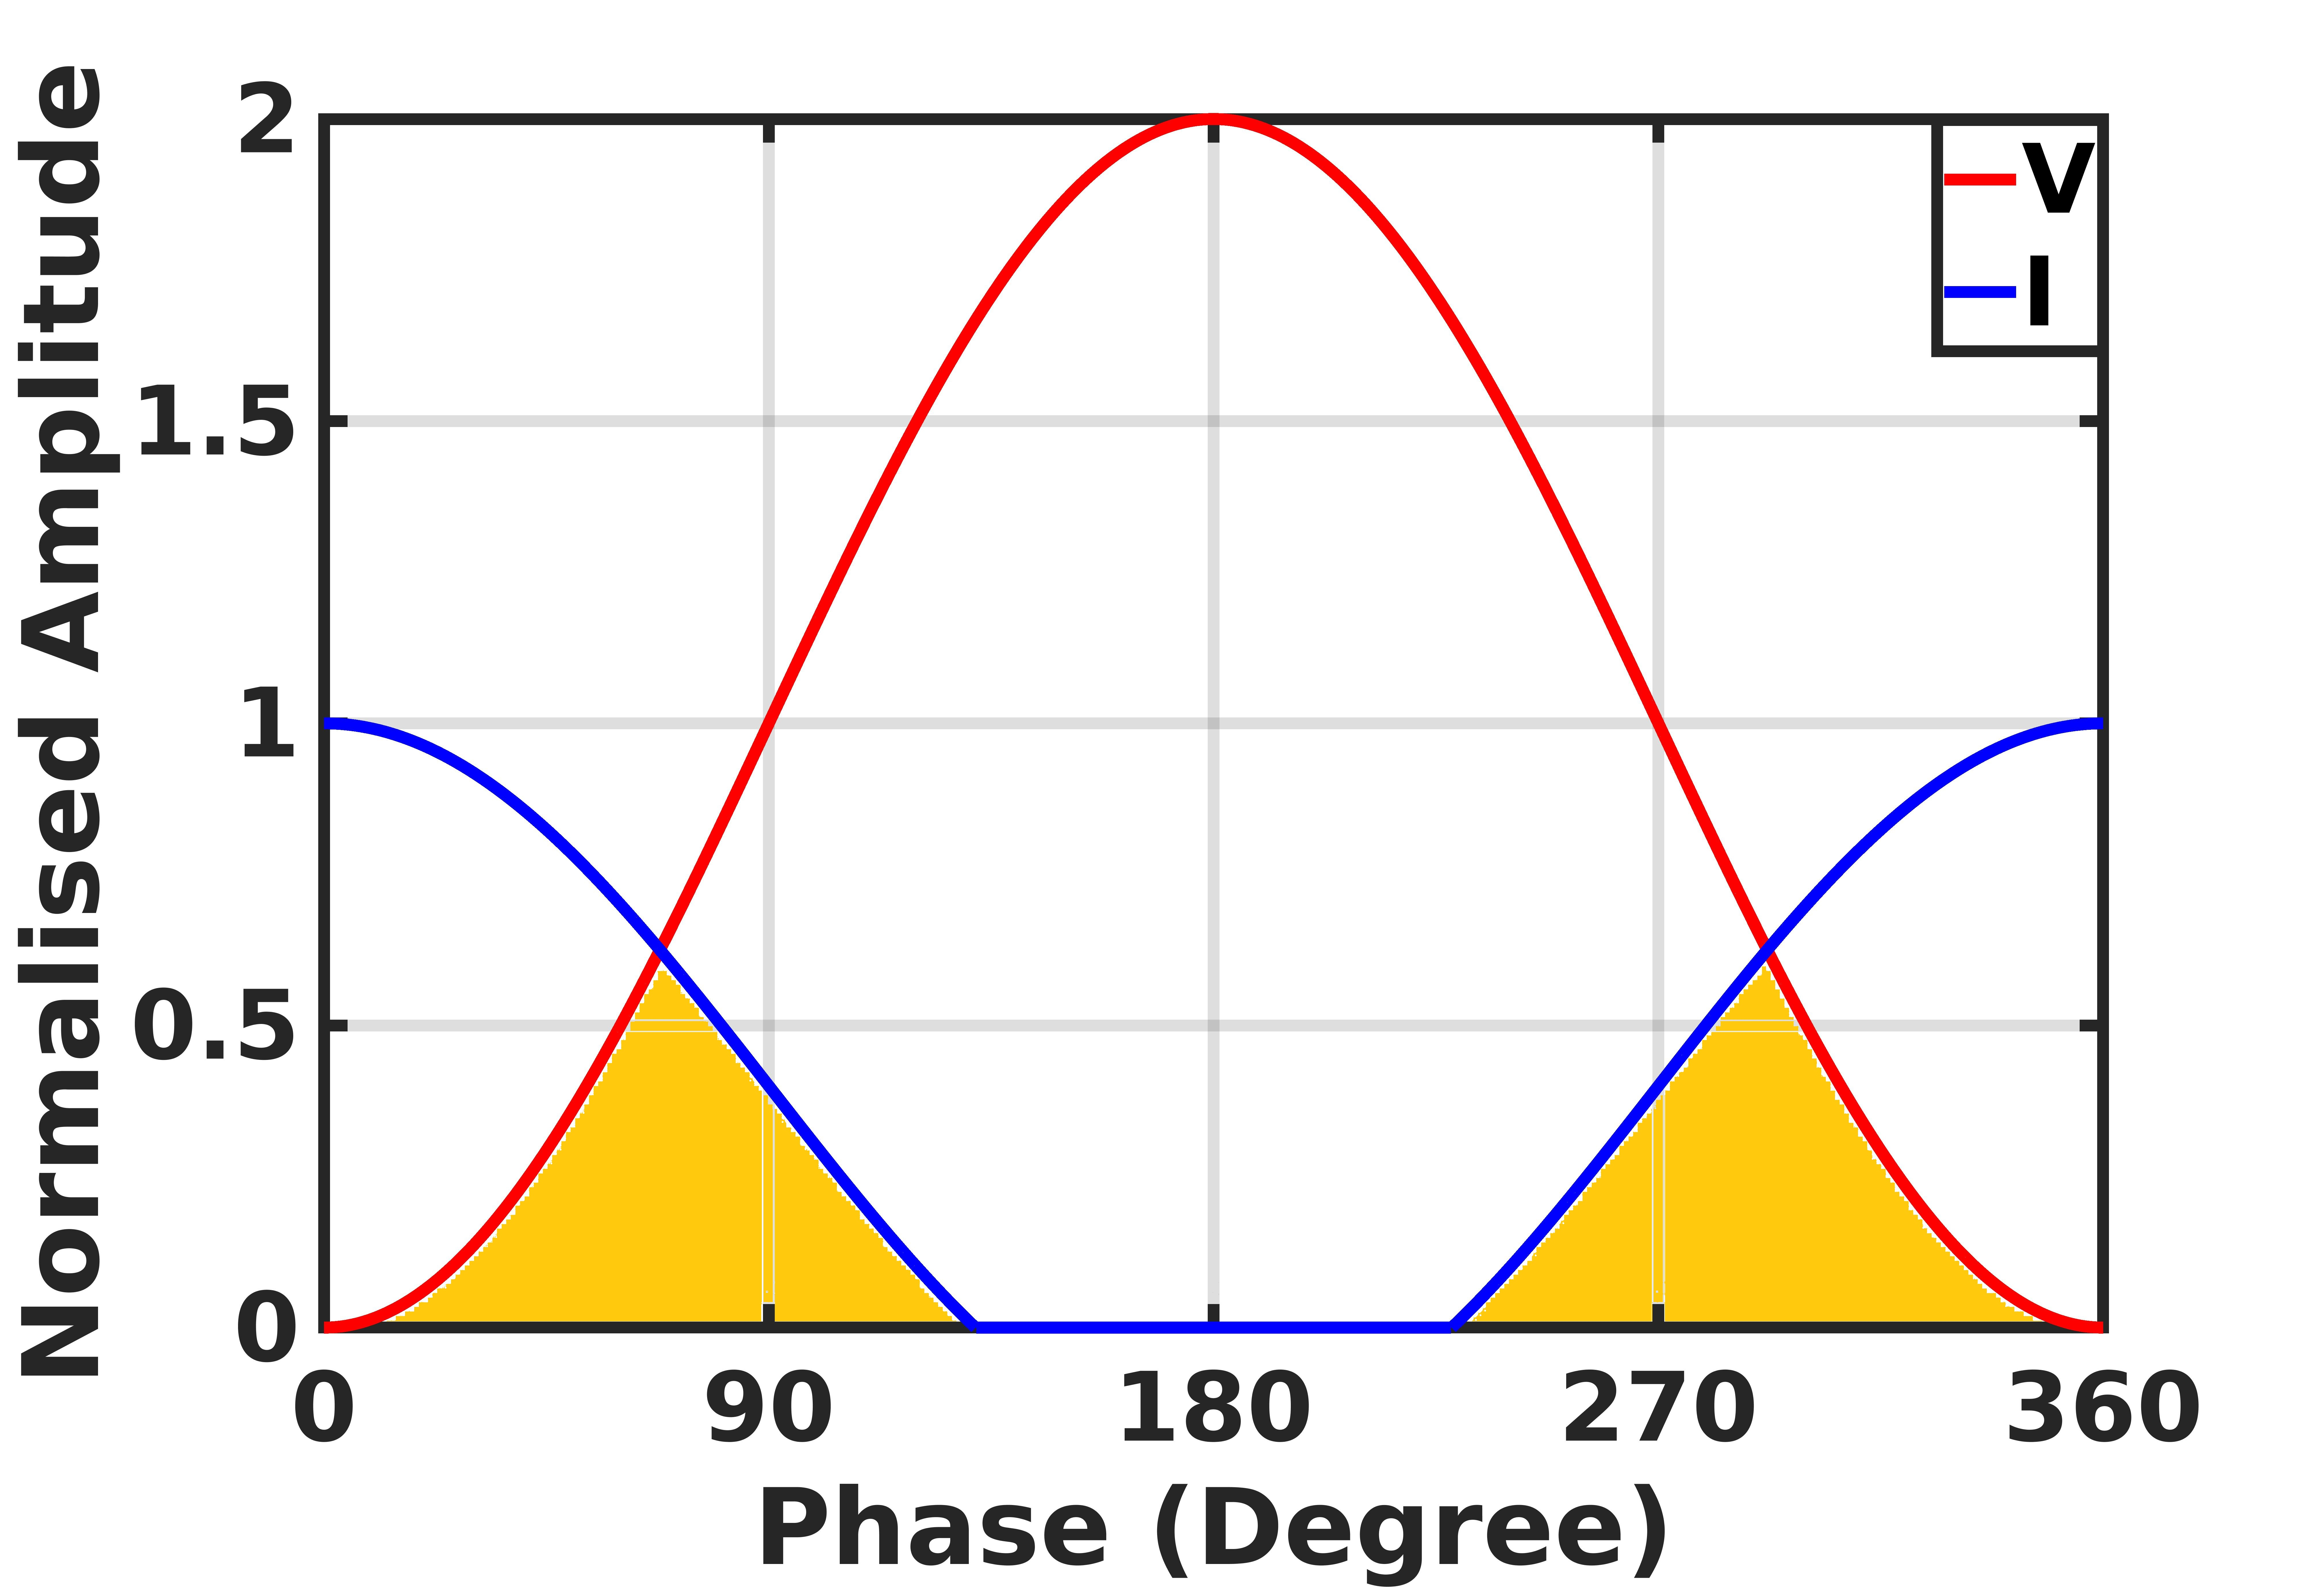
\includegraphics[width=0.9\textwidth]{Images/Intro/ClassB_shaded.jpg}
\caption{Class B}
\label{fig:CB_wave_VI}
\end{subfigure}
\begin{subfigure}{0.24\textwidth}
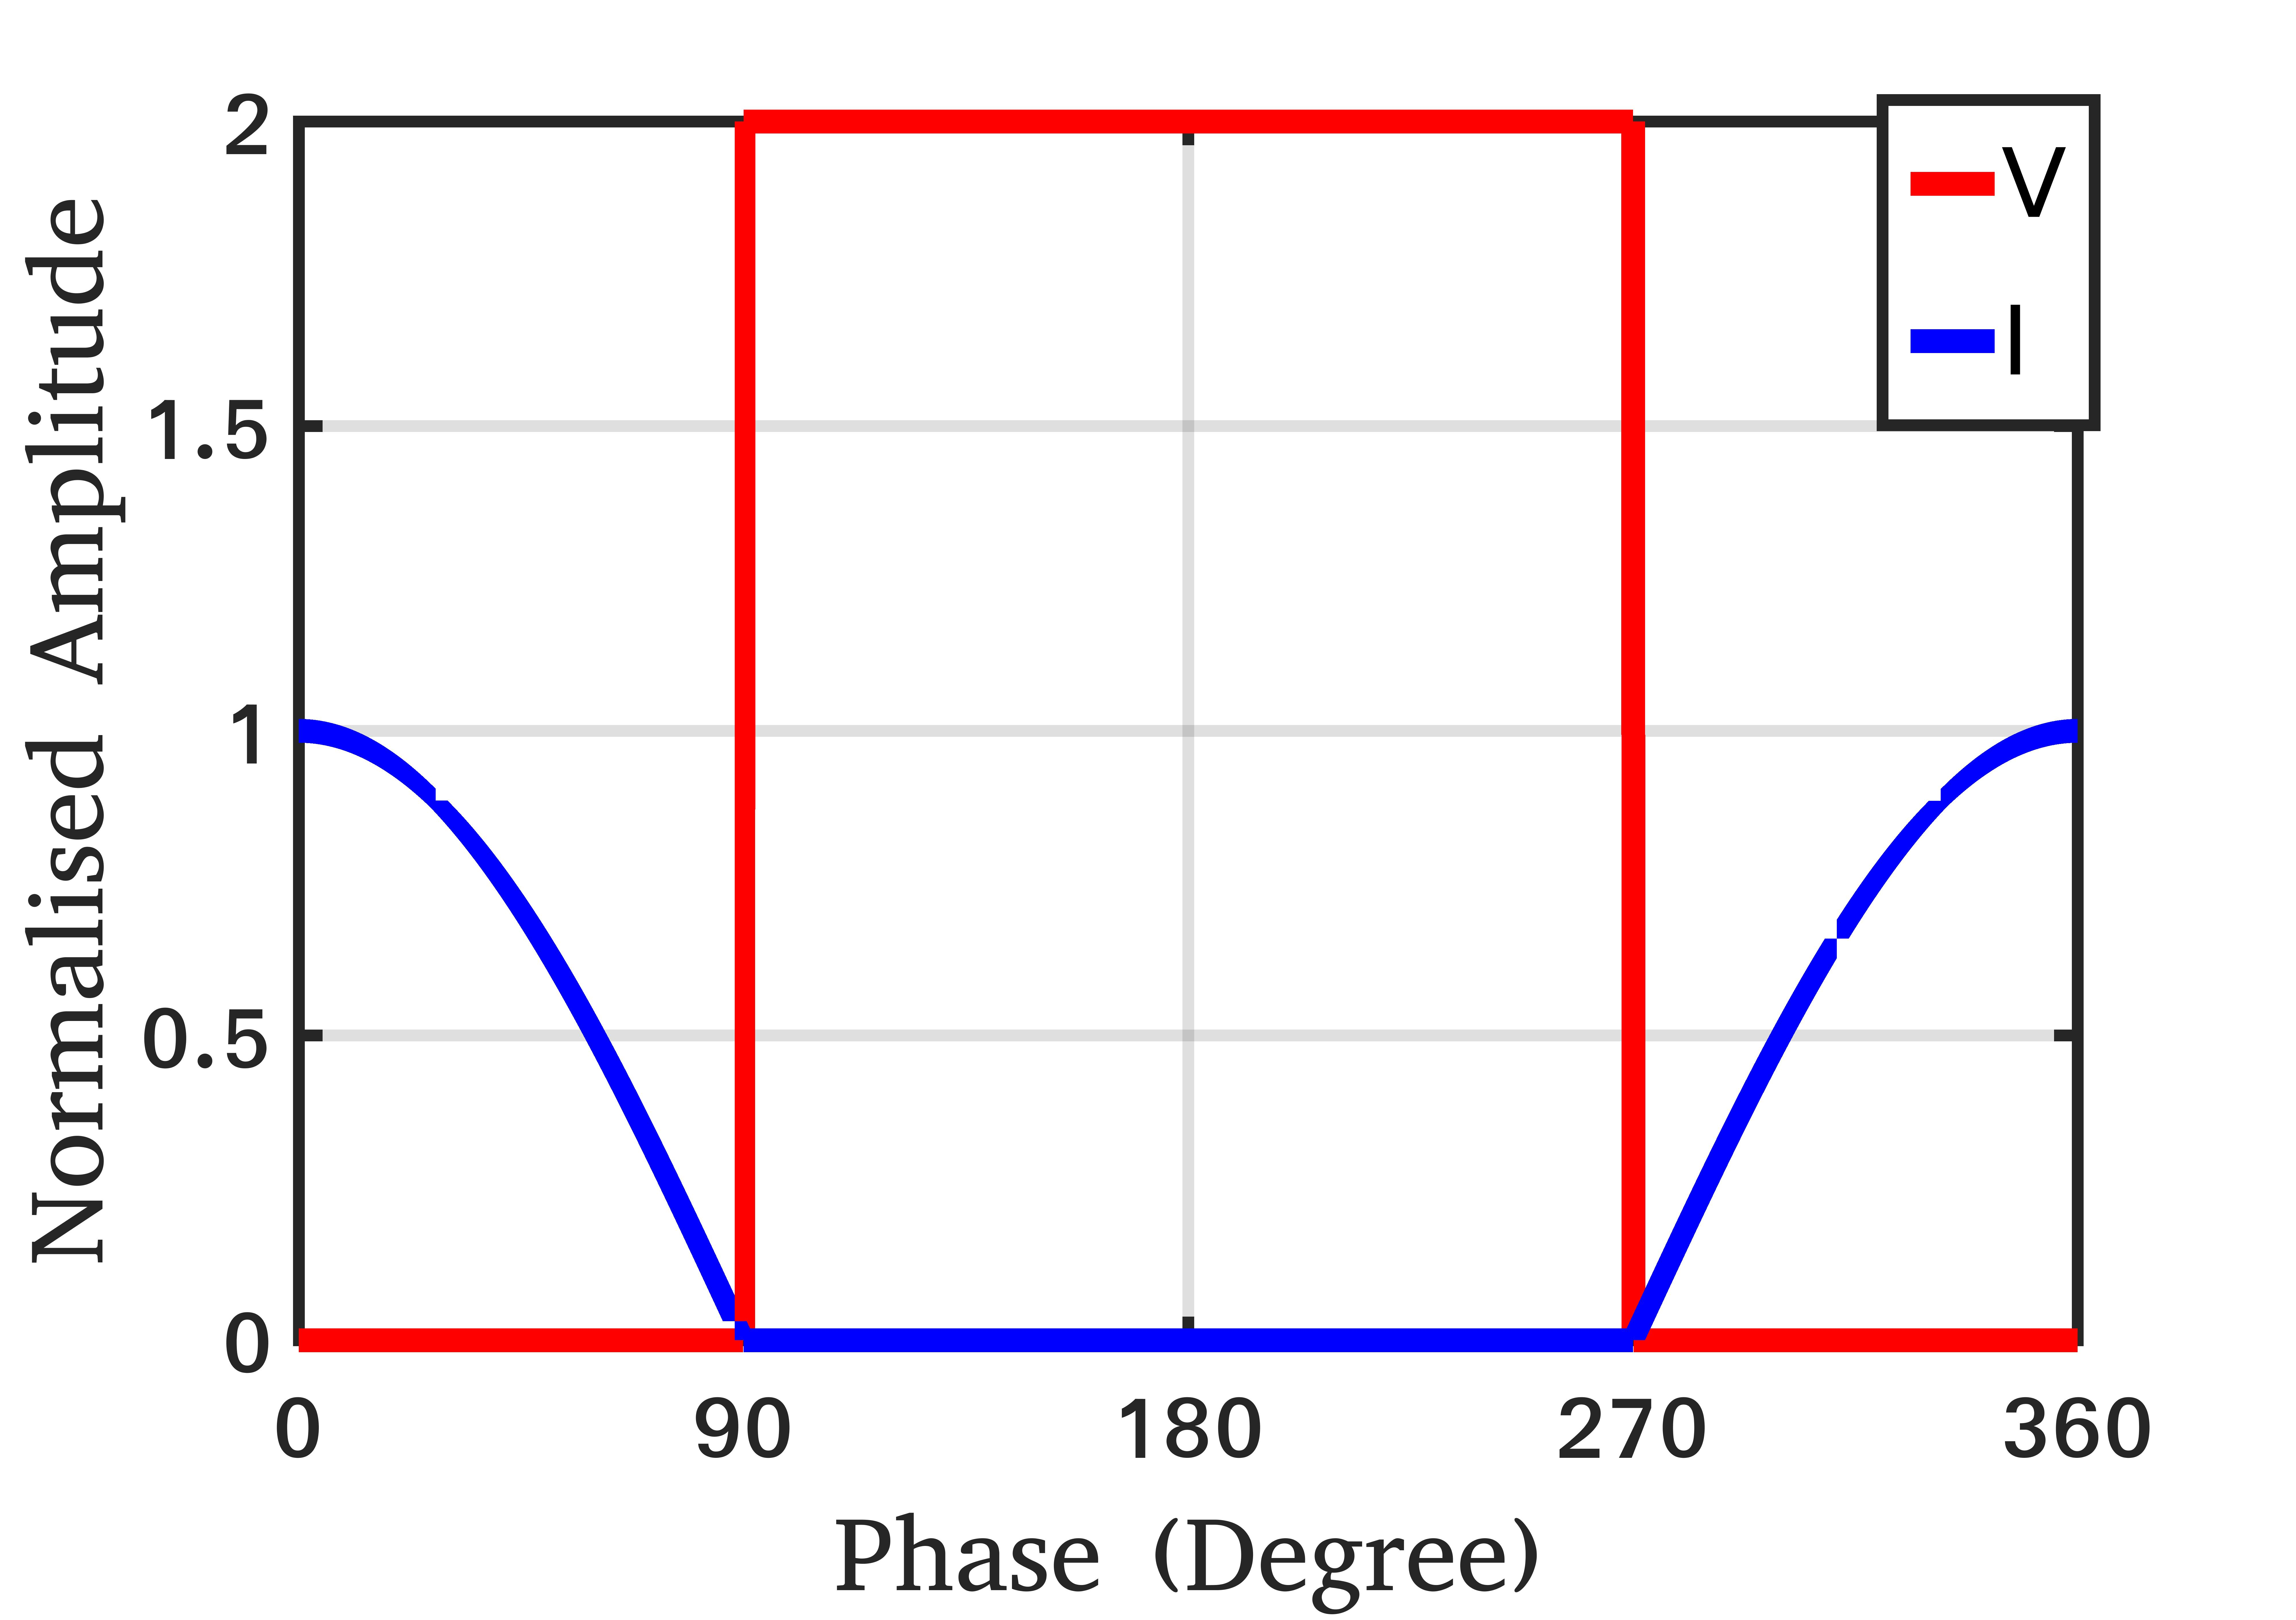
\includegraphics[width=0.9\textwidth]{Images/Intro/ClassF.jpg}
\caption{Ideal Class F}
\label{fig:ICF_wave_VI}
\end{subfigure}
\begin{subfigure}{0.24\textwidth}
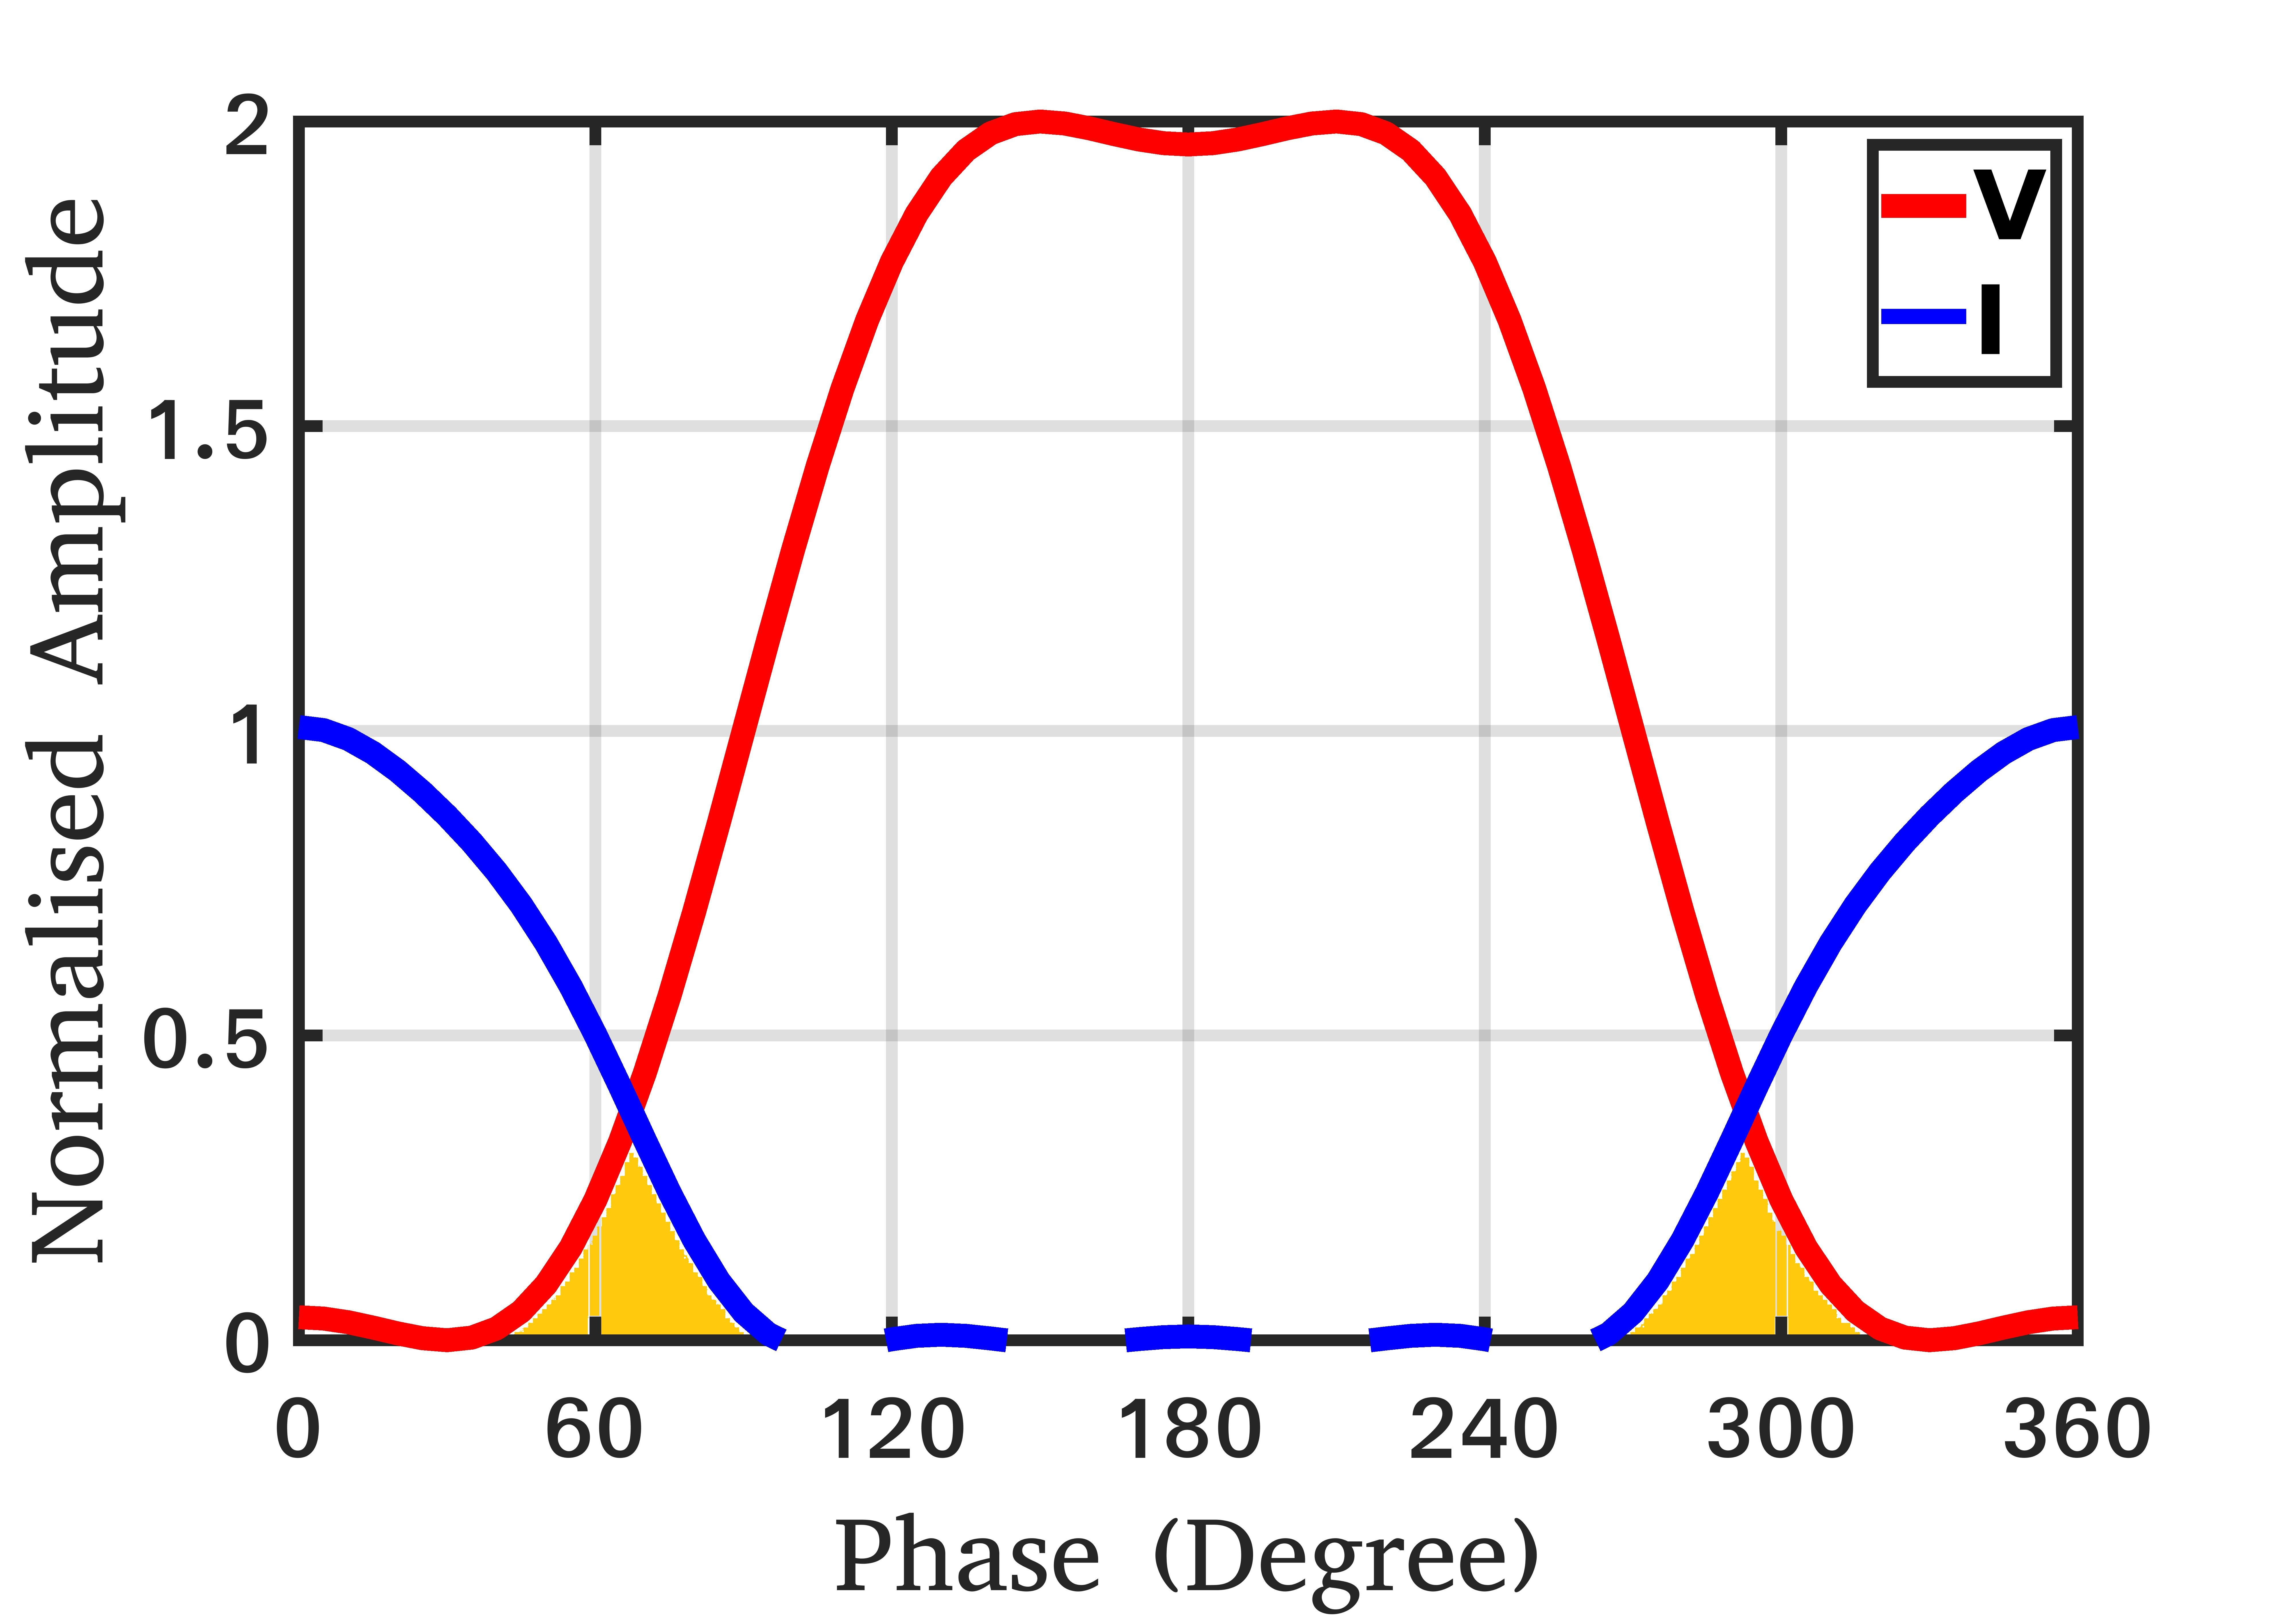
\includegraphics[width=0.9\textwidth]{Images/Intro/CF_wave_VI_shaded.jpg}
\caption{Practical Class F}
\label{fig:CF_wave_VI}
\end{subfigure}
\caption{\color{blue}The class A/B/F drain \color{blue} voltage (V)/current (I) waveforms. \color{black}}
\label{fig:wave_VI}
\vspace{-0.25in}
\end{figure}
Generalized drain source voltage ($V_{DS}$) containing all frequencies up to $3^{rd}$ harmonic \cite{Gen_Vds_eqn} is given by:
\begin{equation}
V_{DS}=\underbrace{1}_{\text{DC}}-\underbrace{\frac{2}{\sqrt{3}} \cos \theta}_{\text{Fundamental}}+\underbrace{\frac{1}{3 \sqrt{3}} \cos 3 \theta}_{\text{$3^{rd}$ harmonic}}
\label{eqn_CF_V}
\end{equation}
Drain current ($I_{D}$) which is a half-sine wave is given by
\begin{equation}
I_{D}=\underbrace{\frac{1}{\pi}}_{\text{DC}}+\underbrace{\frac{1}{2} \cos \theta}_{\text{Fundamental}}+\underbrace{\frac{2}{3 \pi} \cos 2 \theta}_{\text{$2^{nd}$ harmonic}}-\underbrace{\frac{2}{15 \pi} \cos 4 \theta}_{\text{$4^{th}$ harmonic}}
\label{eqn_CCF_I}
\end{equation}
Load impedance in the fundamental, $2^{nd}$ and $3^{rd}$  harmonic bands are represented by $Z_{1f}$, $Z_{2f}$ and $Z_{3f}$ respectively.
\begin{equation}
\begin{aligned}
Z_{1f}=\frac{4}{\sqrt{3}}, \hspace{3mm}
Z_{2f}=0, \hspace{3mm}
Z_{3f}=\infty
\end{aligned}
\label{eqn_CF}
\end{equation}
Figure \ref{fig:CF_wave_VI} shows that the peak factor in class F is \textit{2}. Practical implementation of class F PA has a peak efficiency of \textit{90.7\%} but the main drawback is that they have limited bandwidths (typically \textit{10\%}) owing to the need for short and open circuit harmonic terminations. Thus, to realize wider bandwidth, the CCF PA has been proposed \cite{CCF_reason}.

The Section \ref{section:CCF} explains in brief the equation governing the operation of CCF. This is followed by Section \ref{section:ON} which discusses the procedure to design the different output networks for CCF. Then, the Section \ref{section:Results} comprises of the comparison results of \textit{4} proposed output network designs. Finally, Section \ref{section:Conclusion} concludes this paper.   

\section{Continuous Class F}
\label{section:CCF}
\vspace{-0.05in}
Compared to class F, the CCF has an imaginary part added at the fundamental and $2^{nd}$ harmonic of voltage waveform. So, the generalized $V_{DS}$ for CCF is given by \cite{ECCF_Carrubba}:
\begin{equation}
V_{DS}=\underbrace{1}_{\text{DC}}-\underbrace{\frac{2}{\sqrt{3}} \cos \theta-\gamma \sin \theta}_{\text{Fundamental}}+\underbrace{\frac{7 \gamma}{6 \sqrt{3}} \sin 2 \theta}_{\text{$2^{nd}$ harmonic}}+\underbrace{\frac{1}{3 \sqrt{3}} \cos 3 \theta}_{\text{$3^{rd}$ harmonic}}
\label{eqn_CCF_V}
\end{equation}
$I_{D}$ is a half sinusoid as in class F and given by Equation \ref{eqn_CCF_I}. It is seen that $V_{DS}$ and $I_{D}$ are chosen in such a way that no power is dissipated at higher harmonics. Also, the $\gamma$ in Equation \ref{eqn_CCF_V} doesn’t affect drain efficiency ($\eta_D$) mathematically. But the voltage waveform’s shape (peak factor) depends on $\gamma$ which is depicted in Figure \ref{fig:CCF_wave_VI}. 
But in reality, $I_{D}$ depends on $V_{DS}$, so $\eta_D$ reduces as $\gamma$ increases.

\begin{figure}[!t]
\centering
\captionsetup{font=footnotesize}
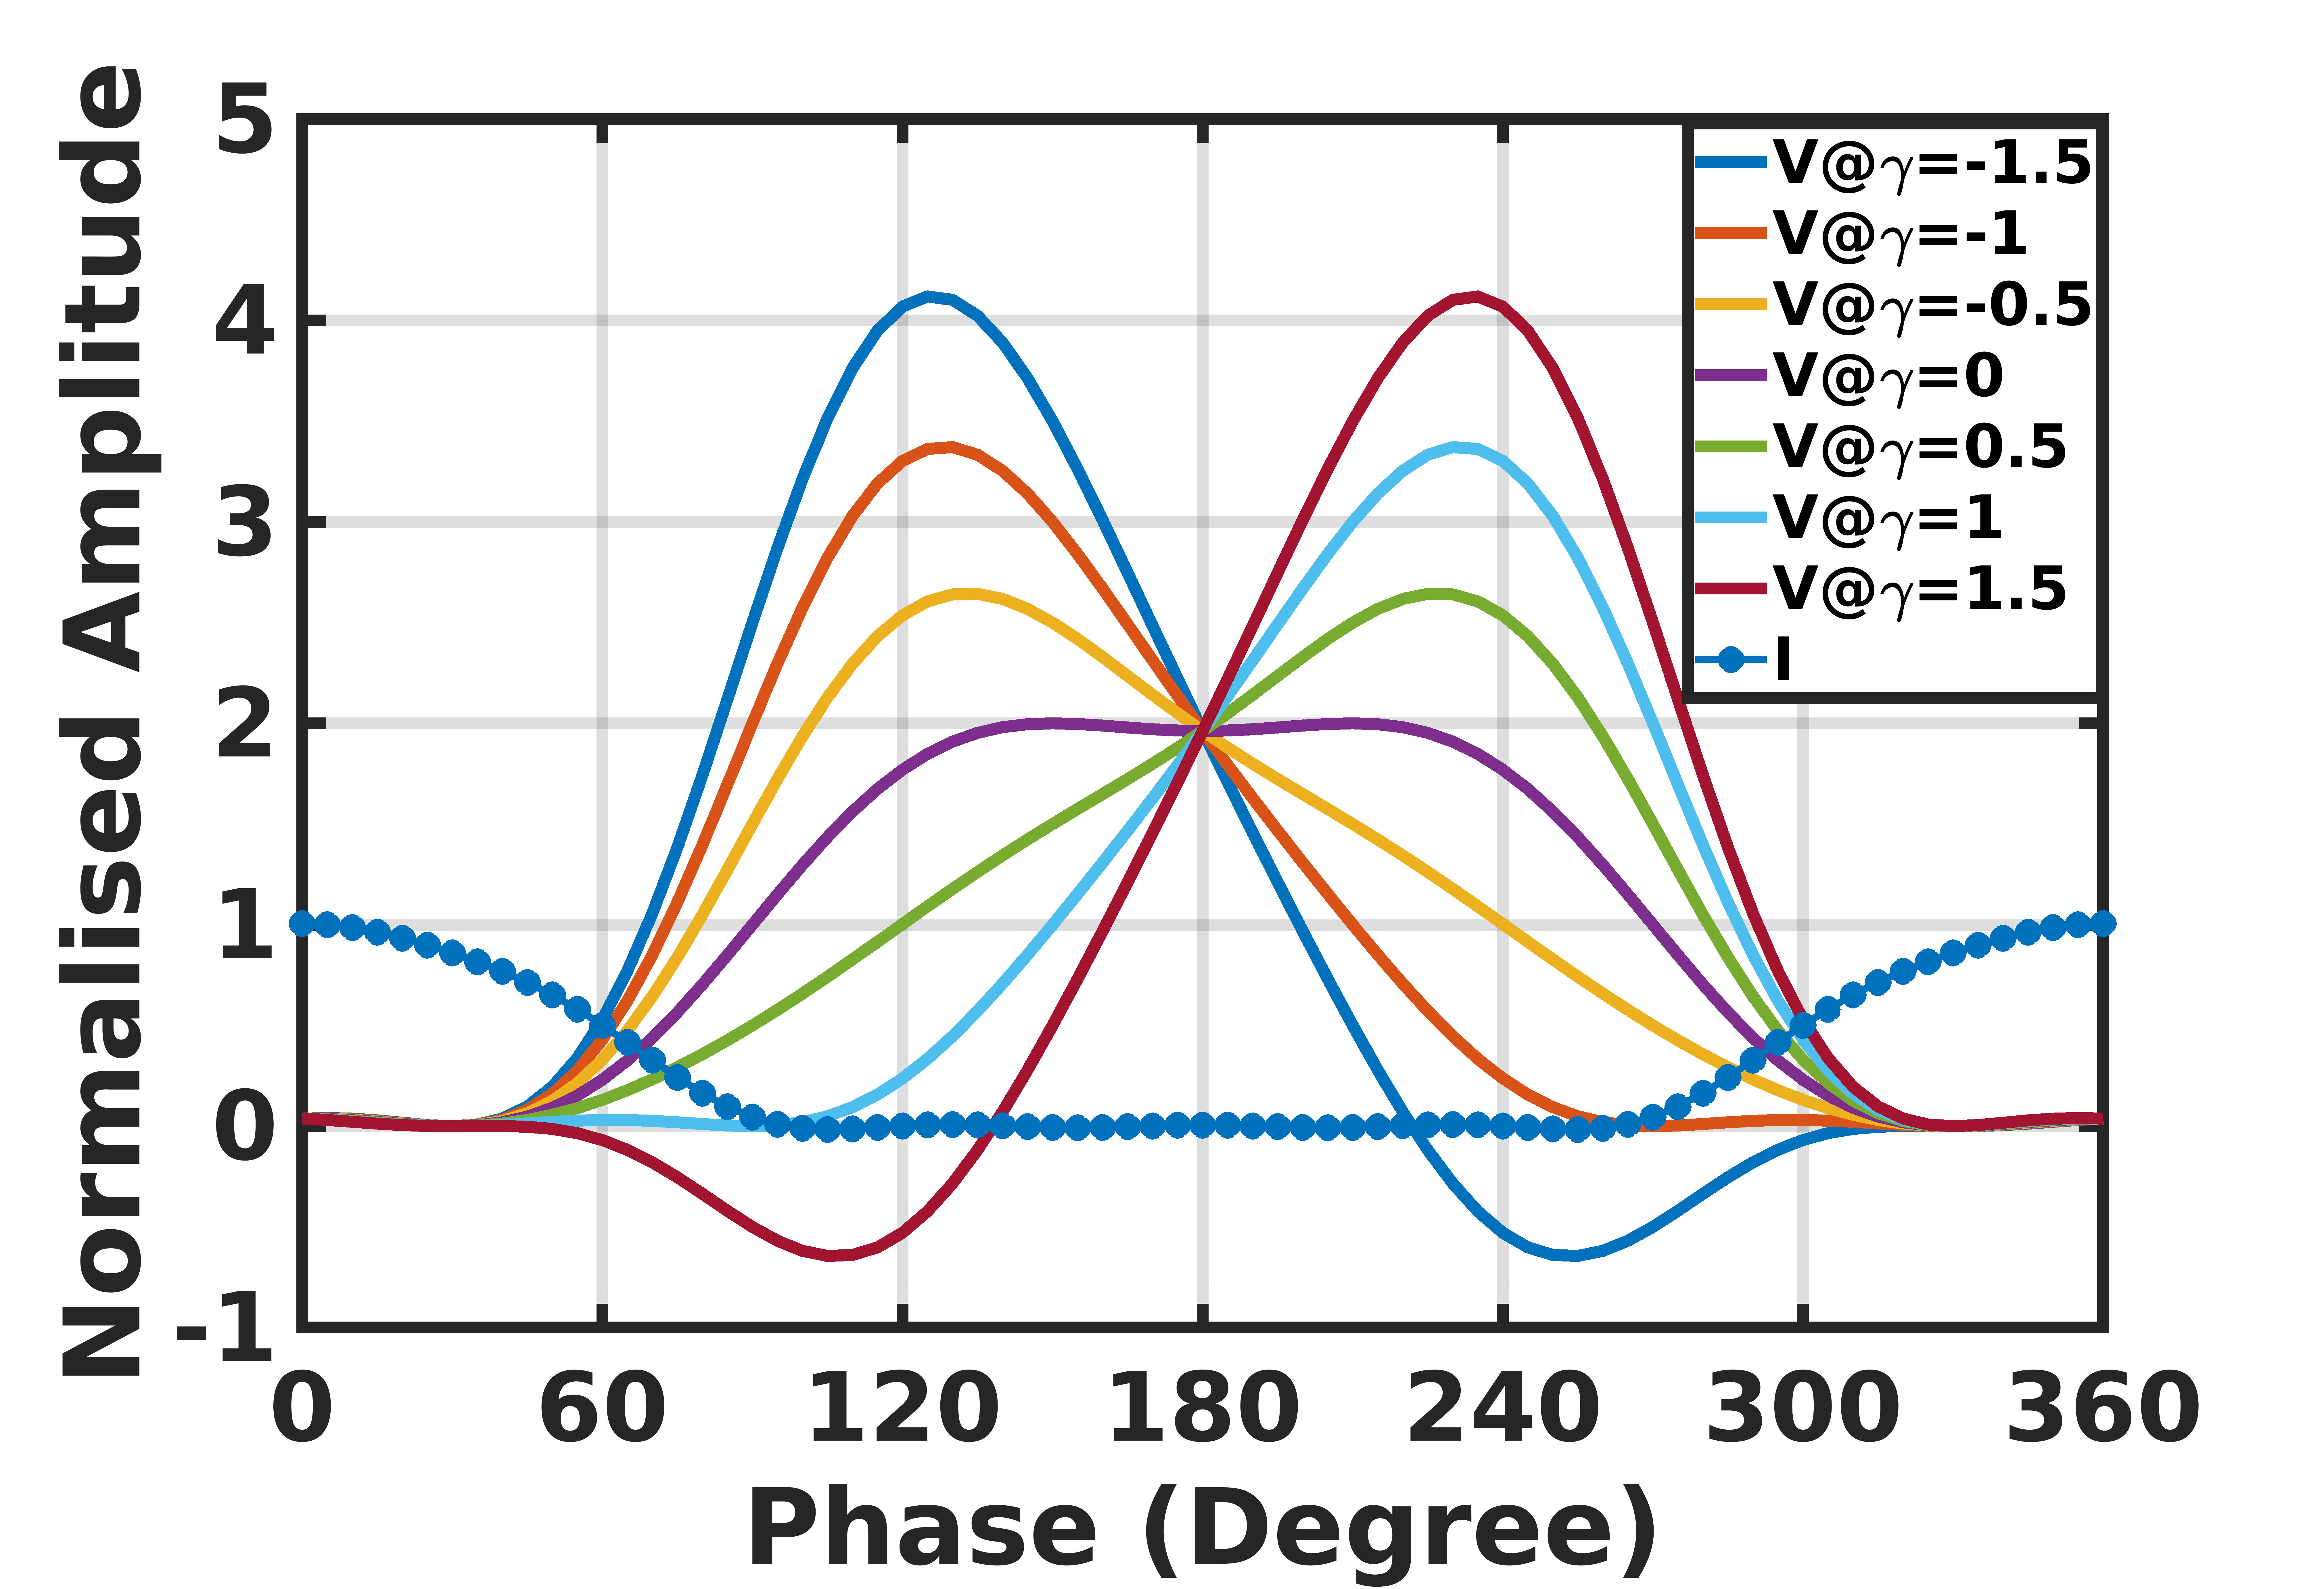
\includegraphics[width=3.4in, height=2in]{Images/CCF/CCF_wave_VI.jpg}
\caption{$V_{DS}$ and $I_D$ waveform for CCF with \textit{-1.5} $<$ $\gamma$ $<$ \textit{1.5}}
\label{fig:CCF_wave_VI}
\vspace{-0.25in}
\end{figure}

Figure \ref{fig:CCF_wave_VI} shows that at $\gamma$ = \textit{0}, waveform is like class F. For the $\gamma$ values between \textit{-1} and \textit{1}, $V_{DS}$ remains positive which enables CCF PA to have good linearity. One of the main downside of CCF PA is the increase in peak factor which reaches a value of \textit{3.12} times the supply ($V_{DD}$) when $\gamma$ = \textit{-1} or \textit{1}. 
Load impedance for CCF are calculated using Equations \ref{eqn_CCF_V} and \ref{eqn_CCF_I} \cite{CCFDesign_ali}.
\begin{equation}
\begin{aligned}
Z_{1f}=\frac{4}{\sqrt{3}}+j 2 \gamma, \hspace{2mm}
Z_{2f}=0-j \frac{\pi}{2} \frac{7 \sqrt{3}}{6} \gamma,\hspace{2mm}
Z_{3f}=\infty
\label{eqn_CCF_imp}
\end{aligned}
\end{equation}

In CCF, $Z_{3f}$ remains open-circuited similar to class F. Meanwhile, $Z_{1f}$ and $Z_{2f}$ has a reactive part, unlike Class F. From the Equation \ref{eqn_CCF_imp} and Figure \ref{fig:CCF_SC}, it is observed that if the reactive part of $Z_{1f}$ changes from inductive to capacitive, then the reactive part of $Z_{2f}$ need to change from capacitive to inductive or vice-versa across the bandwidth to achieve CCF operation. In the next section, the design procedure for the \textit{4} output networks is illustrated step by step.

\begin{figure}[!t]
\centering
\captionsetup{font=footnotesize}
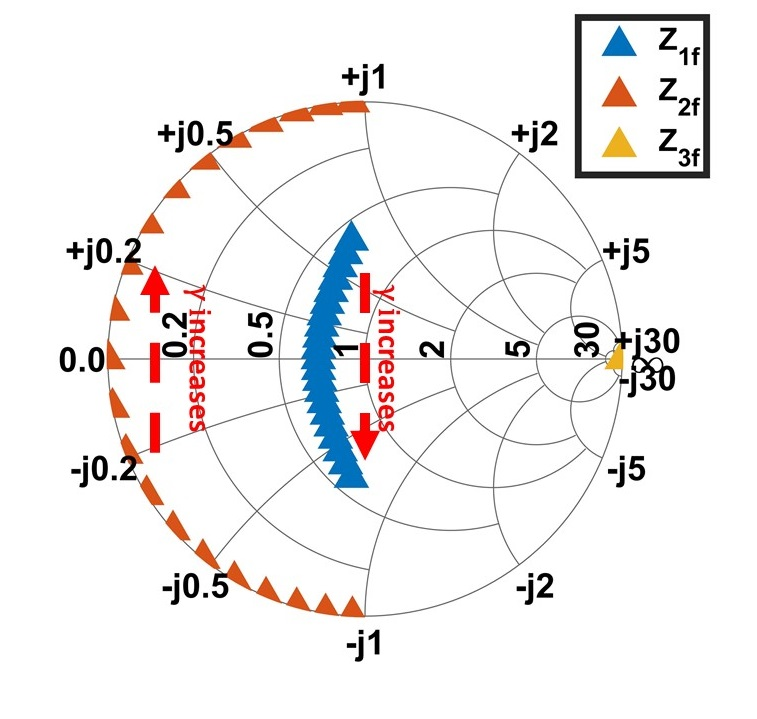
\includegraphics[width=0.8\linewidth]{Images/CCF/CCF_SC.jpg}
\caption{Variation of $Z_{1f}$, $Z_{2f}$, $Z_{3f}$ for \textit{-1} $<$ $\gamma$ $<$ \textit{1}}
\label{fig:CCF_SC}
\vspace{-0.05in}
\end{figure}
 

\section{Design of Output Network for CCF}
\label{section:ON}
In this paper, the differential structure is chosen for the PA mainly because it helps to decouple the design of $2^{nd}$ harmonic impedance with the fundamental and $3^{rd}$ harmonic impedance. Moreover, it also helps to reduce common-mode noise, substrate coupling, and second-order nonlinearities as well as double the output power compared to single-ended. 
The PA in this paper is designed for a peak power of \textit{27 dBm} for the operational bandwidth of \textit{2.1 - 2.7 GHz} with $V_{DD}$ = \textit{2.7 V} and to achieve this, a differential impedance of \textit{38.7} $\Omega$ should be presented to the drains of the transistors at fundamental across the entire bandwidth (refer Equation \ref{eqn_diff_imp}). 
\vspace{-0.1in}
\begin{equation}
\begin{aligned}
&V_{FUND}(de)=2*V_{FUND}(se)=2*\frac{2}{\sqrt{3}} V_{DD}=6.24 \hspace{1mm}V\\
&R_{D}(de)=\frac{V_{FUND}(de)^{2}}{2*\text{Peak} \hspace{1mm} P_{OUT}}=38.7 \hspace{1mm} \Omega
\label{eqn_diff_imp}
\end{aligned}
\end{equation}
The requirements of the output network for CCF is exhibited in Table \ref{tab:Output_Network_Requirements}. The PA operates in Class F mode at the center frequency $\omega_0$ (\textit{2.4 GHz}) with a short at $2\omega_0$ (\textit{4.8 GHz}) and an open at $3\omega_0$ (\textit{7.2 GHz}). But, for all other frequencies, the PA performs in the CCF mode. 

\setlength{\arrayrulewidth}{0.5mm}
\setlength{\tabcolsep}{2pt}
\renewcommand{\arraystretch}{1.5}
\begin{table}[!t]
\centering
\captionsetup{font=footnotesize}
\resizebox{\linewidth}{!}{%
\begin{tabular}{|c|c|c|c|}
\hline
\textbf{Class of Operation} & \begin{tabular}[c]{@{}c@{}}\textbf{First Harmonic} ($\omega$)\end{tabular} & \begin{tabular}[c]{@{}c@{}}\textbf{Second Harmonic} (2$\omega$)\end{tabular} & \begin{tabular}[c]{@{}c@{}}\textbf{Third Harmonic} (3$\omega$)\end{tabular} \\ \hline
\multirow{2}{*}{\textbf{\begin{tabular}[c]{@{}c@{}}Class F \\ (2.4 GHz)\end{tabular}}} & $\Re(Z_D)$ = 38.7 $\Omega$ & $\Re(Z_D)$= 0 $\Omega$ & \multirow{2}{*}{\begin{tabular}[c]{@{}c@{}}$|Z_D|$ needs to be high \end{tabular}} \\ \cline{2-3}
 & $\Im(Z_D)$ = 0 $\Omega$ & $\Im(Z_D)$ = 0 $\Omega$ &  \\ \hline
\multirow{2}{*}{\textbf{\begin{tabular}[c]{@{}c@{}}\\CCF \\ (2.1 - 2.7 GHz)\end{tabular}}} & $\Re(Z_D)$ = 38.7 $\Omega$ & $\Re(Z_D)$ = 0 $\Omega$ & \multirow{2}{*}{\begin{tabular}[c]{@{}c@{}}\\$|Z_D|$ needs to be high \end{tabular}} \\ \cline{2-3}
 & \begin{tabular}[c]{@{}c@{}}$\Im(Z_D)$ need to change from + to -\\ OR\\ $\Im(Z_D)$ need to change from - to +\end{tabular} & \begin{tabular}[c]{@{}c@{}} $\Im(Z_D)$ need to change from - to +\\ OR\\ $\Im(Z_D)$ need to change from + to -\end{tabular} &  \\ \hline
\end{tabular}%
 }
\caption{Output network specifications}
\label{tab:Output_Network_Requirements}
\vspace{-0.25in}
\end{table}

Figures \ref{fig:Design_A_FC}, \ref{fig:Design_B_FC}, \ref{fig:Design_C_FC}, and \ref{fig:Design_D_FC} shows the schematics of \textit{4} output networks which are designed using lossless lumped components.. 
All the designs have a balun and a load capacitance ($C_L$), because the balun converts differential-ended signal to single-ended signal as the load is single-ended, whereas $C_L$ shorts the $R_L$ (\textit{50} $\Omega$) at $3^{rd}$ harmonic to obtain high impedance. Drain source capacitance of the transistor (Assumed $C_{DS}=1.87\hspace{1mm}pF$) is absorbed into the output network to reduce its impact on the PA performance. The balun is modelled using ideal transformer, magnetizing inductance ($L_m$), leakage inductance ($L_k$), primary inductance ($L_P$) and coupling coefficient ($km$) \cite{Transformer_model}. 

\subsection{Design A (no RF choke \& with $L_2C_2$)}
Design A consists of a second harmonic trap ($L_2C_2$) which provides short at $2\omega_0$. The $V_{DD}$ is provided through the center tap of the balun and $L_{BND}$ is used to model bond-wire inductance ($\approx$ \textit{1 nH}).
Analysis of the schematics is done in differential and common mode by using the equivalent circuit shown in Figure \ref{fig:Design_A_Diff} and \ref{fig:Design_A_Com} respectively to calculate the unknown parameters: $km$, transformer's turn ratio ($N$), $L_P$, $C_2$, $L_2$, and $C_L$.
\begin{figure}[!t]
\captionsetup{font=footnotesize}
\centering
\begin{subfigure}{0.5\textwidth}
\centering
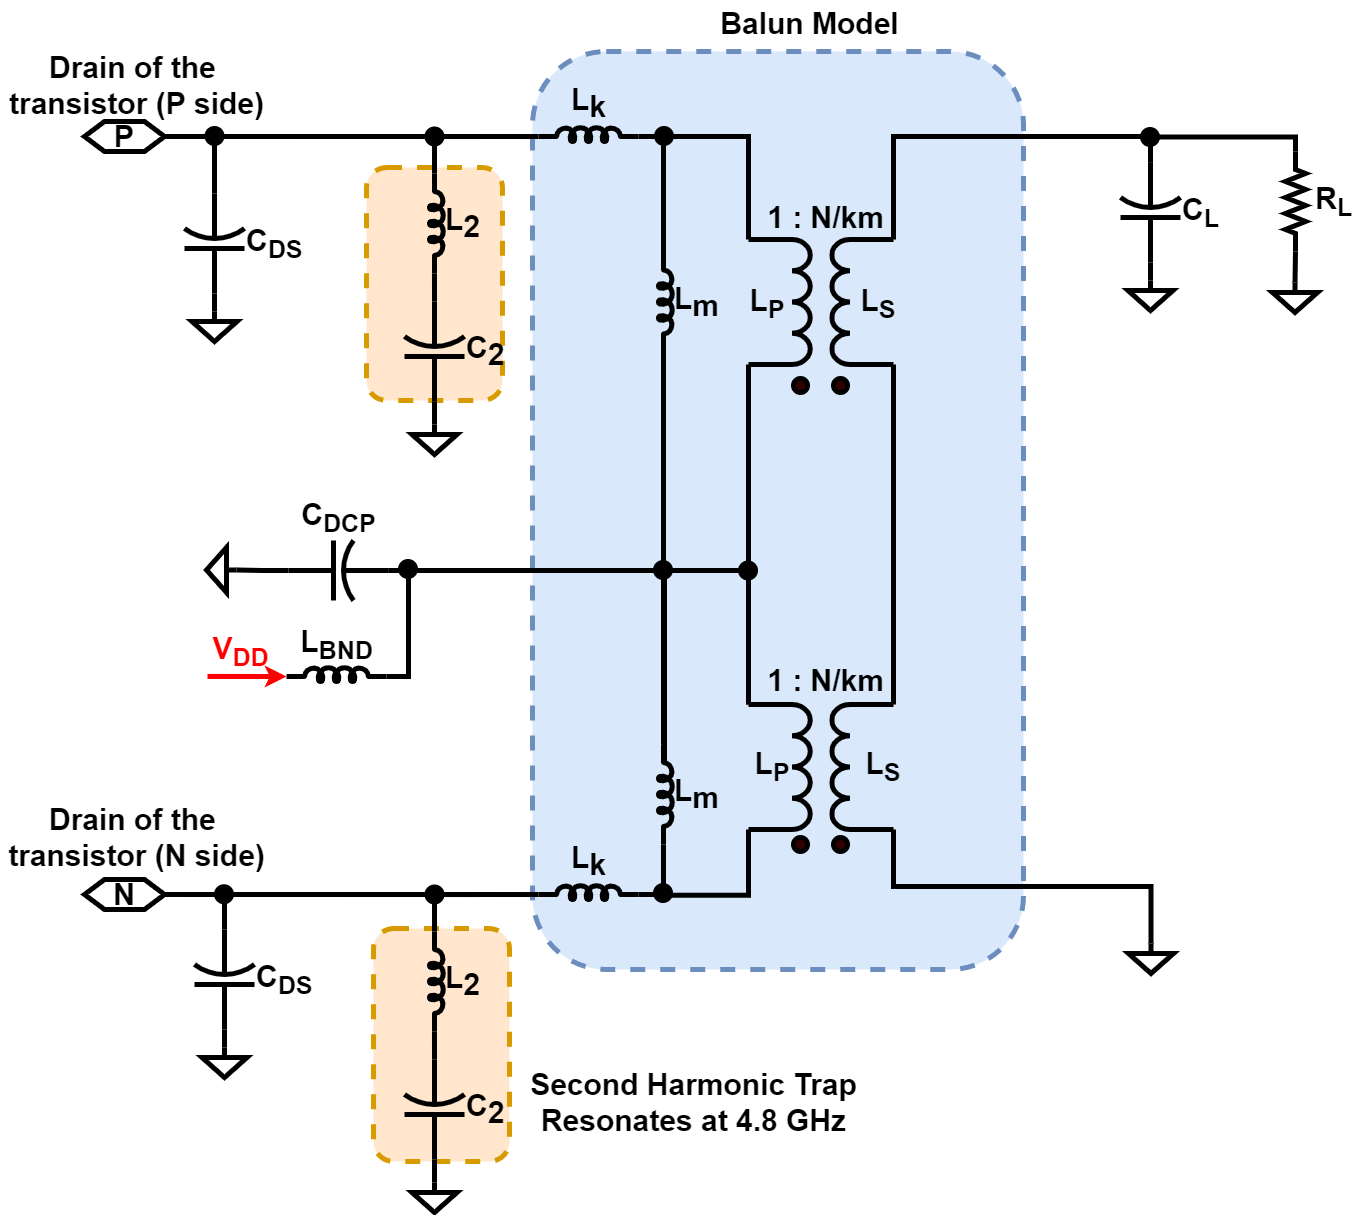
\includegraphics[width=0.5\textwidth]{Images/Design/Design_A_FC.png}
\caption{Schematics}
\label{fig:Design_A_FC}
\end{subfigure}
\begin{subfigure}[b]{0.24\textwidth}
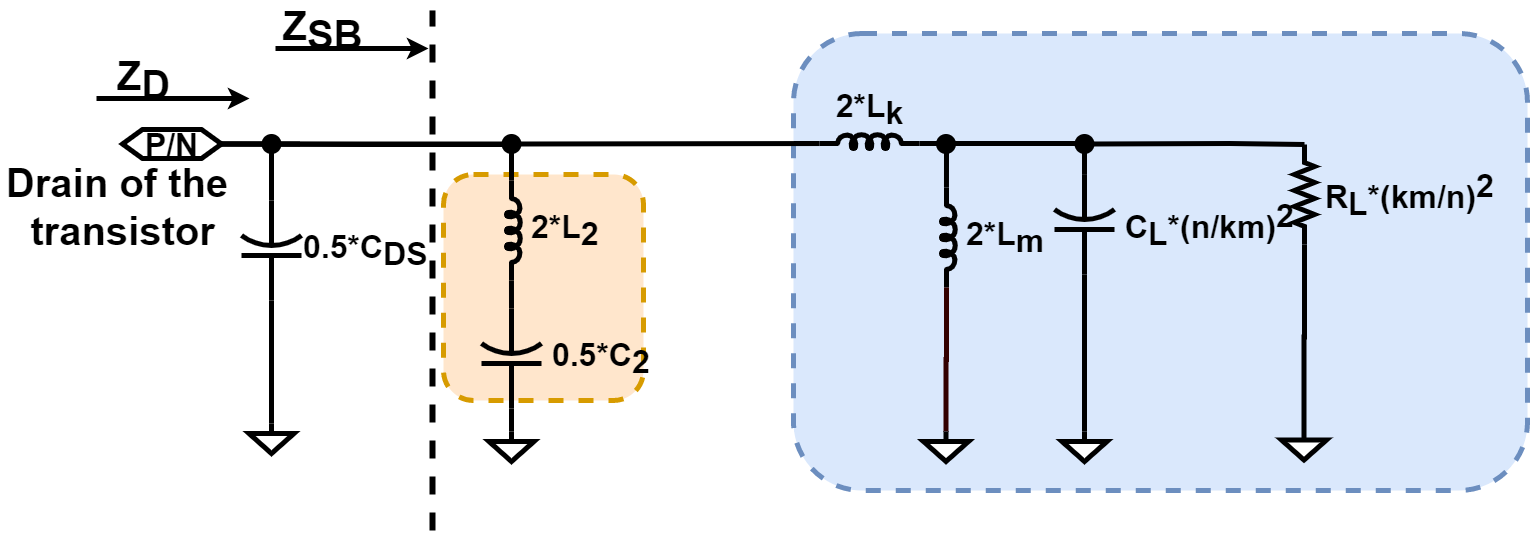
\includegraphics[width=1\textwidth]{Images/Design/Design_A_Diff.png}
\caption{Differential mode equivalent circuit}
\label{fig:Design_A_Diff}
\end{subfigure}
\begin{subfigure}[b]{0.24\textwidth}
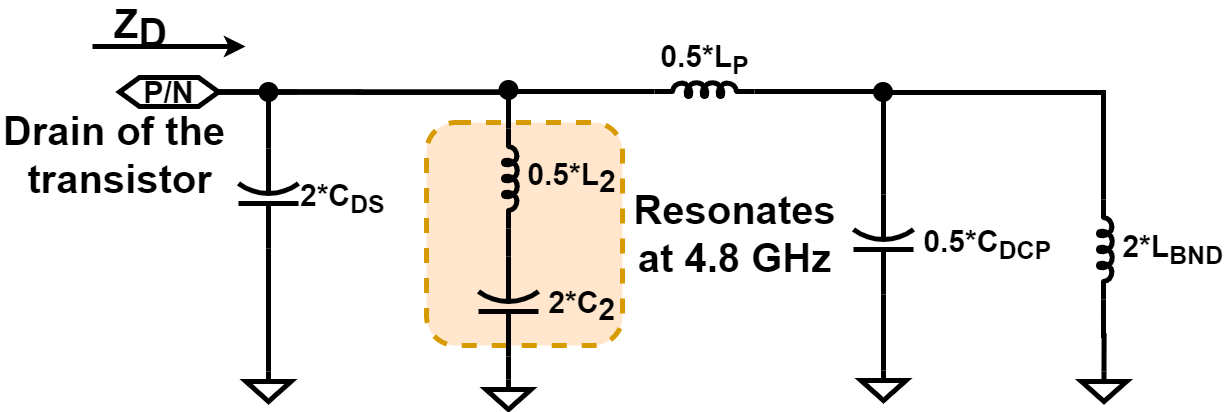
\includegraphics[width=1\textwidth]{Images/Design/Design_A_Com.png}
\caption{Common mode equivalent circuit}
\label{fig:Design_A_Com}
\end{subfigure}
\caption{Design A (Balun, $L_2C_2$ and $C_L$)}
\label{fig:Design_A}
\vspace{-0.3in}
\end{figure}
Figure \ref{fig:Design_A_Diff} shows that the drain impedance ($Z_D$) is given by
\begin{equation}
    Z_D=(\frac{1}{\frac{j\omega C_{DS}}{2}}+\frac{1}{Z_{SB}})^{-1}=38.7 \hspace{1mm} \Omega
    \label{eqn:ZD}
\end{equation}
The value of $Z_{SB}$ (impedance of $L_2C_2$ and balun given by equation \ref{eqn:Design_A_ZSB}) that will provide $Z_D$ of \textit{38.7} $\Omega$ can be calculated from equation \ref{eqn:ZD} and the value is $\Re(Z_{SB})(\omega_0) =  29.8\hspace{1mm} \Omega$ and $\Im(Z_{SB})(\omega_0) = 16.6\hspace{1mm}\Omega$.

\begin{equation}
\begin{aligned}
    &Z_{SB}=(\frac{1}{Z_B}+\frac{1}{Z_S})^{-1}
    \hspace{1mm}\text{where}, Z_S=2j\omega  L_2+\frac{1}{\frac{j \omega C_2}{2}}, \\
    &Z_B=(\frac{1}{R_P}+\frac{1}{2j \omega  L_m}+j \omega C_P)^{-1}+2j \omega  L_k,\\ &R_P=R_L(\frac{km}{n})^2,C_P=C_L(\frac{n}{km})^2
\label{eqn:Design_A_ZSB}
\end{aligned}
\end{equation}

From equation \ref{eqn:ZD}, it is evident that $C_{DS}$ should resonate out with $\Im(Z_{SB})$  to attain high drain impedance at $3\omega_0$. This implies $\Im(Z_{SB})(3\omega_0) = 24.96\hspace{1mm}\Omega$.
Ideally, $\Re(Z_{SB})(3\omega_0)$ should be \textit{0} to achieve high $3^{rd}$ harmonic impedance, but Figure \ref{fig:Design_A_Rn_var_1H} depicts that having a larger $\Re(Z_{SB)}(3\omega_0)$ helps to get a constant $P_{OUT}$ across the operational bandwidth by having a flatter real part at the fundamental. Another benefit is that it has more linear reactive part at the fundamental which helps in CCF operation.
However, this leads to a lower $3^{rd}$ harmonic impedance as showcased in Figure \ref{fig:Design_A_Zn_3H}. This also emphasizes  the significance of $C_L$. So, to achieve \textit{1000} $\Omega$ at $3^{rd}$ harmonic,  $\Re(Z_{SB})(3\omega_0) = 0.5\hspace{1mm}\Omega$ which is obtained from Figure \ref{fig:Design_A_Zn_3H}. Figure \ref{fig:Design_A_Com} proves that $L_2$ should  should have a series resonance with $C_2$ to get short at 2$\omega_0$.

\begin{equation}
    L_2=\frac{1}{4*\omega_0^2*C_2}%=0.73 \hspace{1mm} nH
    \label{eqn:Design_A_2H}
\end{equation}

\begin{figure}[!t]
\captionsetup{font=footnotesize}
\centering
\begin{subfigure}{0.24\textwidth}
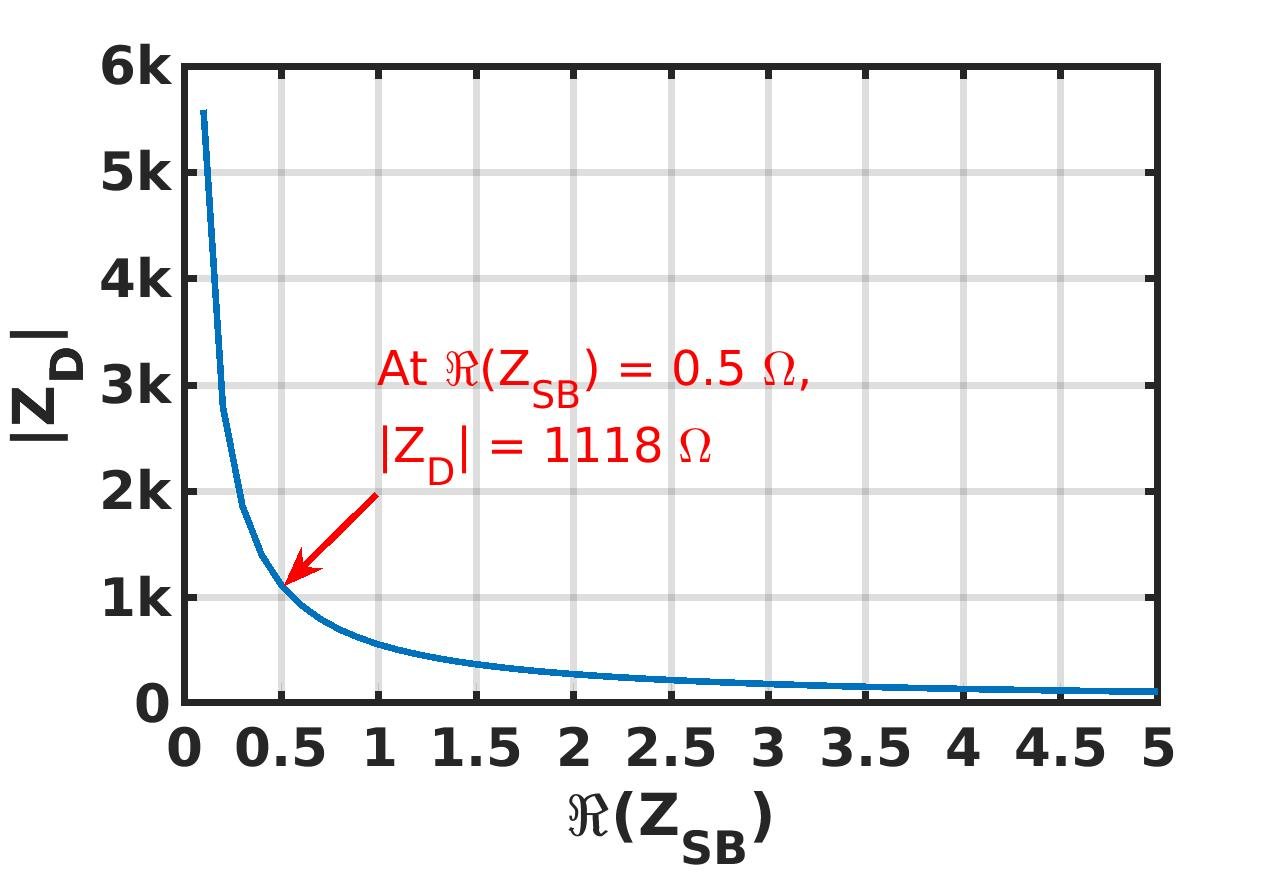
\includegraphics[width=1\textwidth]{Images/Design/Design_A_Zn_3H.jpg}
\caption{}
\label{fig:Design_A_Zn_3H}
\end{subfigure}
\begin{subfigure}{0.24\textwidth}
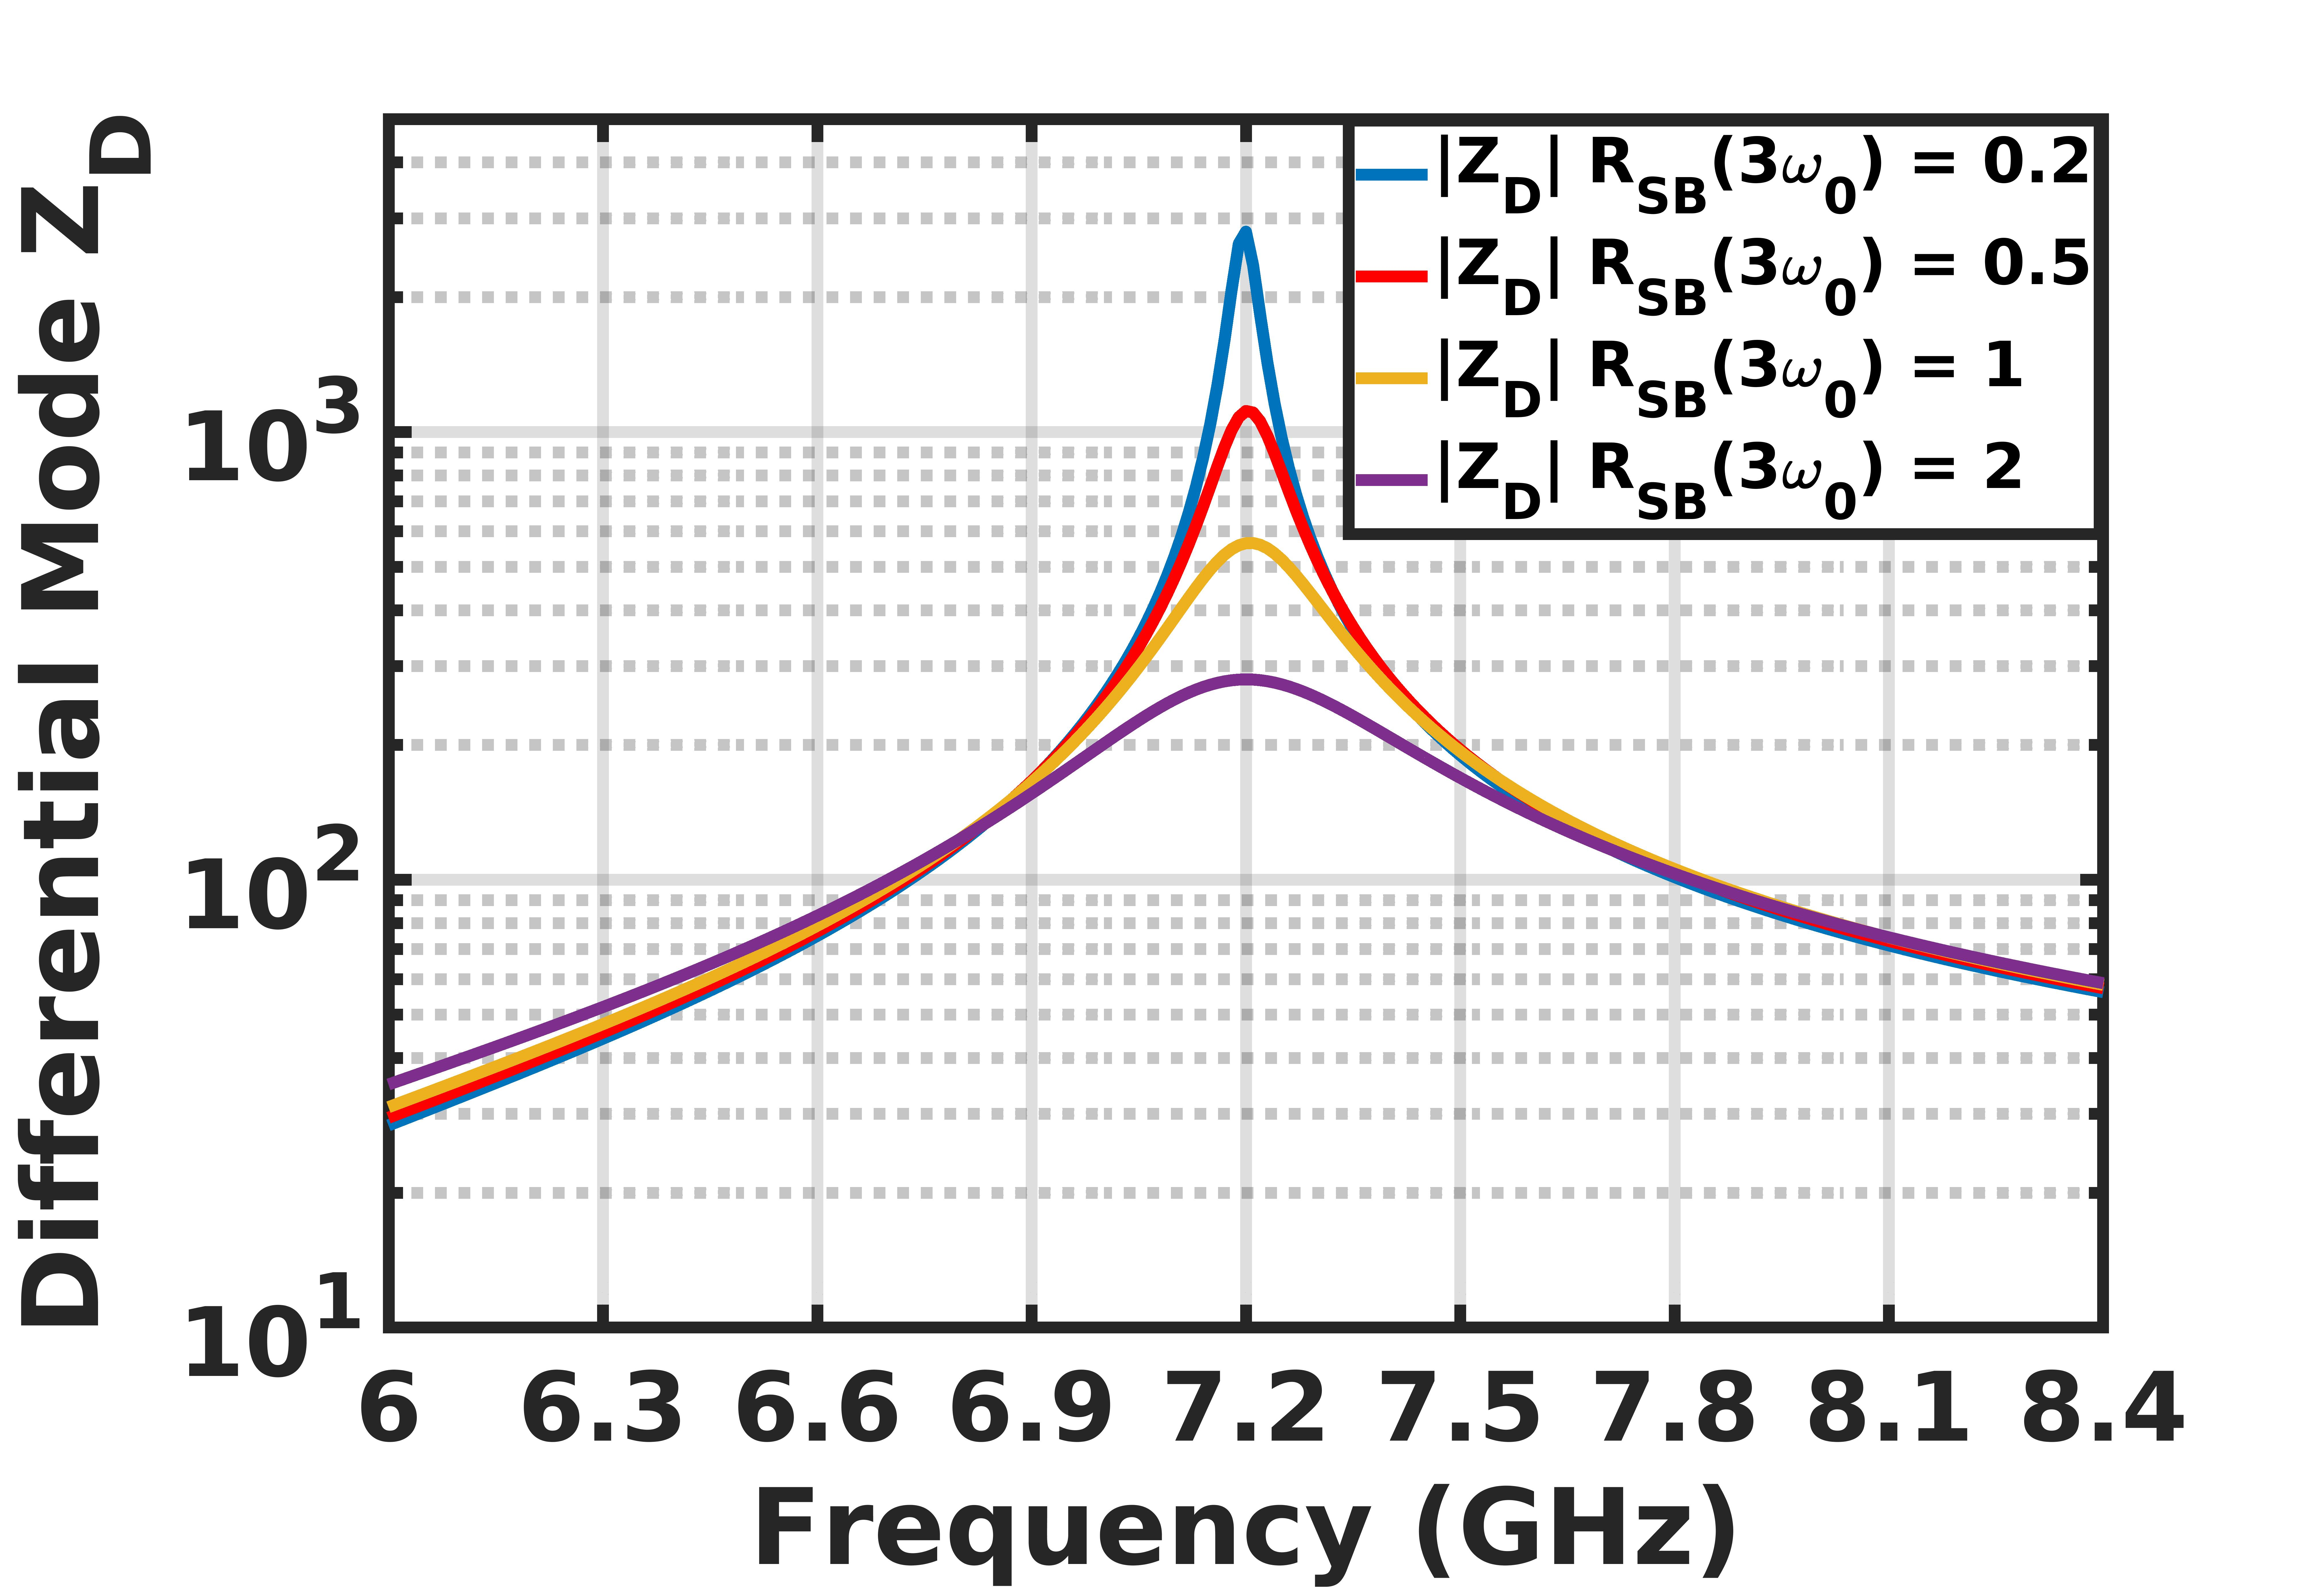
\includegraphics[width=1\textwidth]{Images/Design/Design_A_Rn_var_3H.jpg}
\caption{}
\label{fig:Design_A_Rn_var_3H}
\end{subfigure}
\begin{subfigure}{0.4\textwidth}
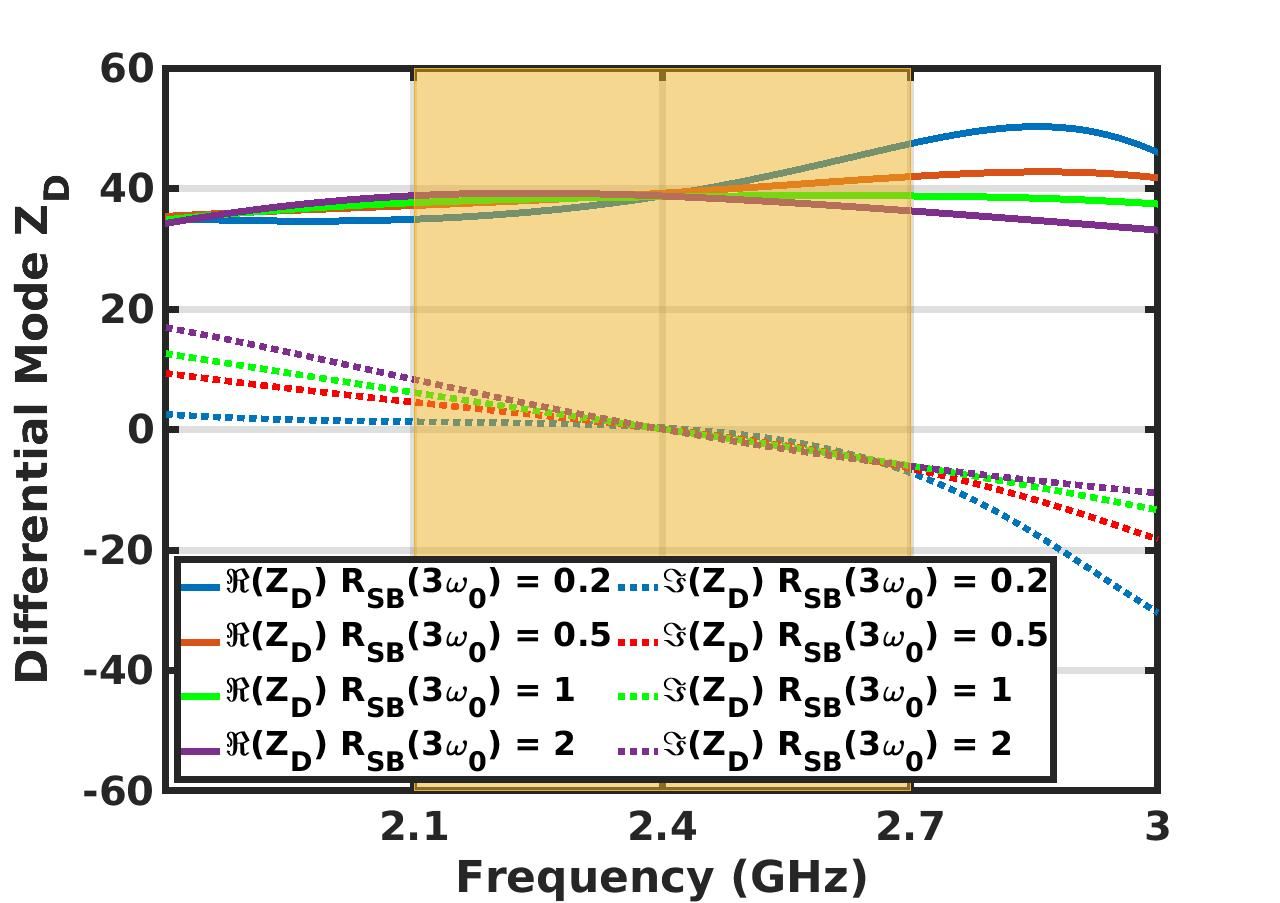
\includegraphics[width=1\textwidth]{Images/Design/Design_A_Rn_var_1H.jpg}
\caption{}
\label{fig:Design_A_Rn_var_1H}
\end{subfigure}
\caption{(a) Magnitude of $Z_{D}$ vs $\Re(Z_{SB})$ at $3\omega_0$; (b) Magnitude of $Z_D$ at $3^{rd}$ harmonic for different $R_{SB}(3\omega_0)$; (c) $Z_D$ at fundamental for different $R_{SB}(3\omega_0)$}
\label{fig:Design_A_Rn_var}
\end{figure}

The \textit{5} unknowns in the circuit: $km$, $N$, $L_P$, $C_2$, and $C_L$ can be calculated by assuming one of them and using \textit{4} equations ($\Re(Z_{SB})(\omega_0) =  29.8\hspace{1mm} \Omega$, $\Im(Z_{SB})(\omega_0) = 16.6\hspace{1mm}\Omega$, $\Re(Z_{SB})(3\omega_0) = 0.5\hspace{1mm}\Omega$ and  $\Im(Z_{SB})(3\omega_0) = 24.96\hspace{1mm}\Omega$). In this paper, $km =$ \textit{0.8} is assumed and the remaining unknowns ($N =$ \textit{1.34}, $L_P =$ \textit{2.2 nH}, $C_L =$ \textit{0.9 pF}, $C_2 =$ \textit{1.5 pF}, $L_2 =$ \textit{0.73 nH}) are calculated. The $km$ can be varied to get different sets of results in which $L_P$ is minimal and thereby making it layout friendly.


\subsection{Design B (no RF choke \& no $L_2C_2$)}

\begin{figure}[!t]
\captionsetup{font=footnotesize}
\centering
\begin{subfigure}{0.24\textwidth}
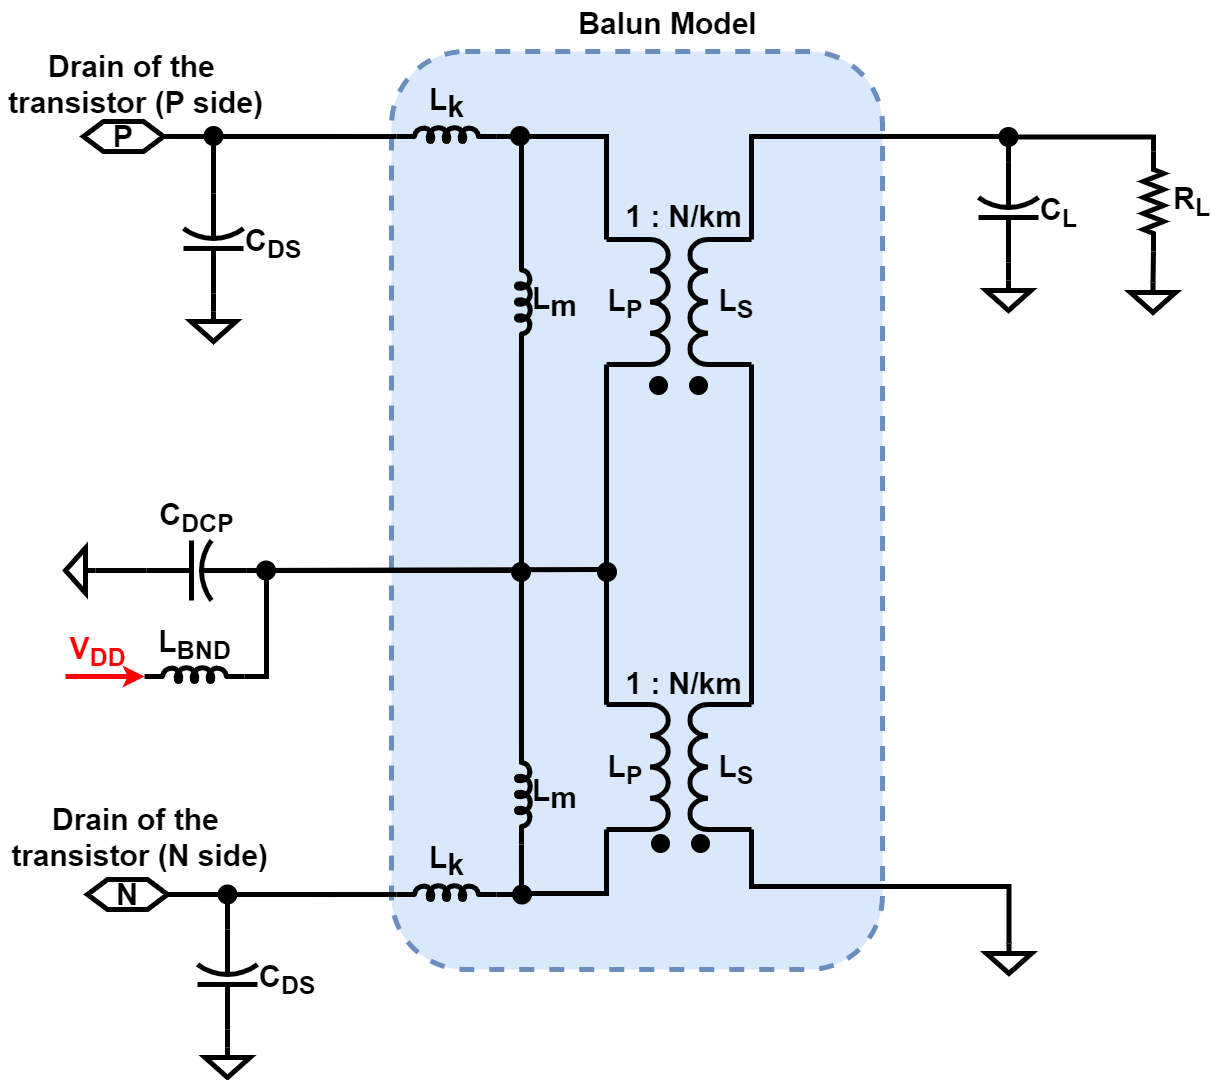
\includegraphics[width=1\textwidth]{Images/Design/Design_B_FC.png}
\caption{}
\label{fig:Design_B_FC}
\end{subfigure}
\begin{subfigure}{0.24\textwidth}
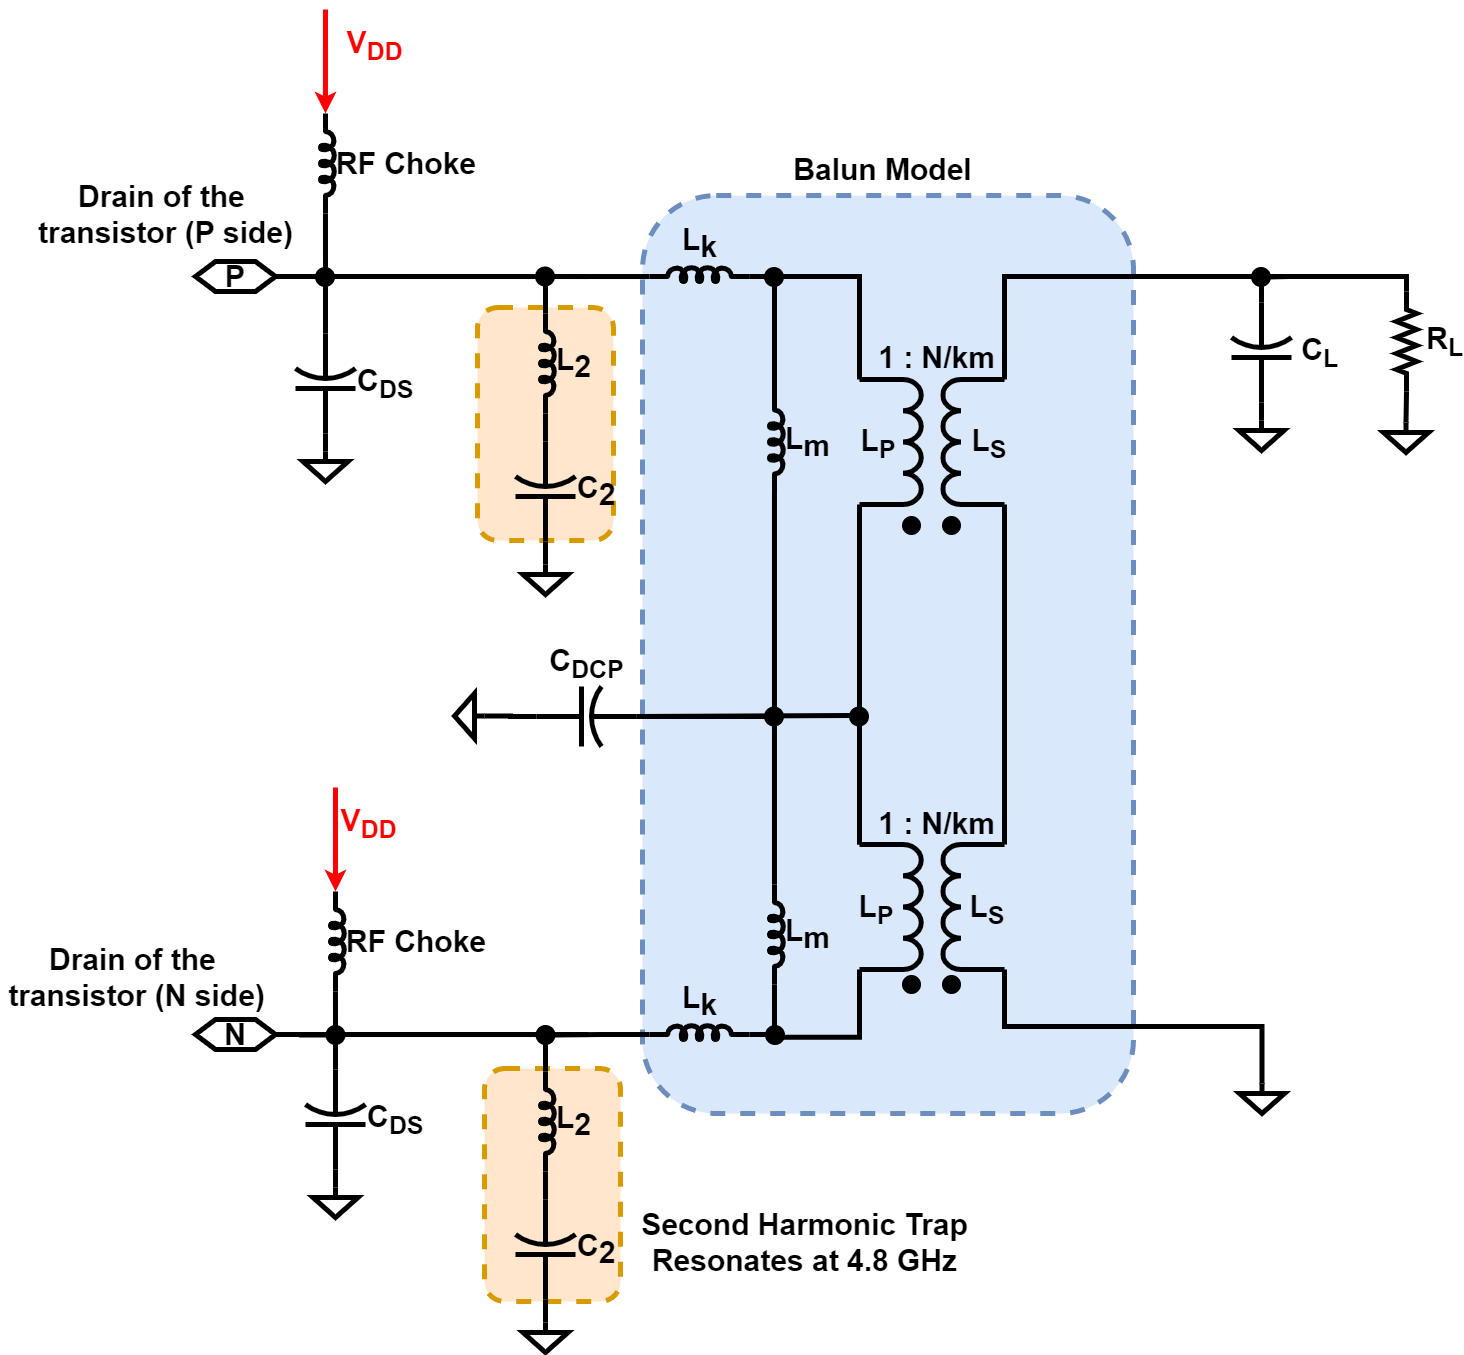
\includegraphics[width=1\textwidth]{Images/Design/Design_C_FC.png}
\caption{}
\label{fig:Design_C_FC}
\end{subfigure}
\begin{subfigure}{0.24\textwidth}
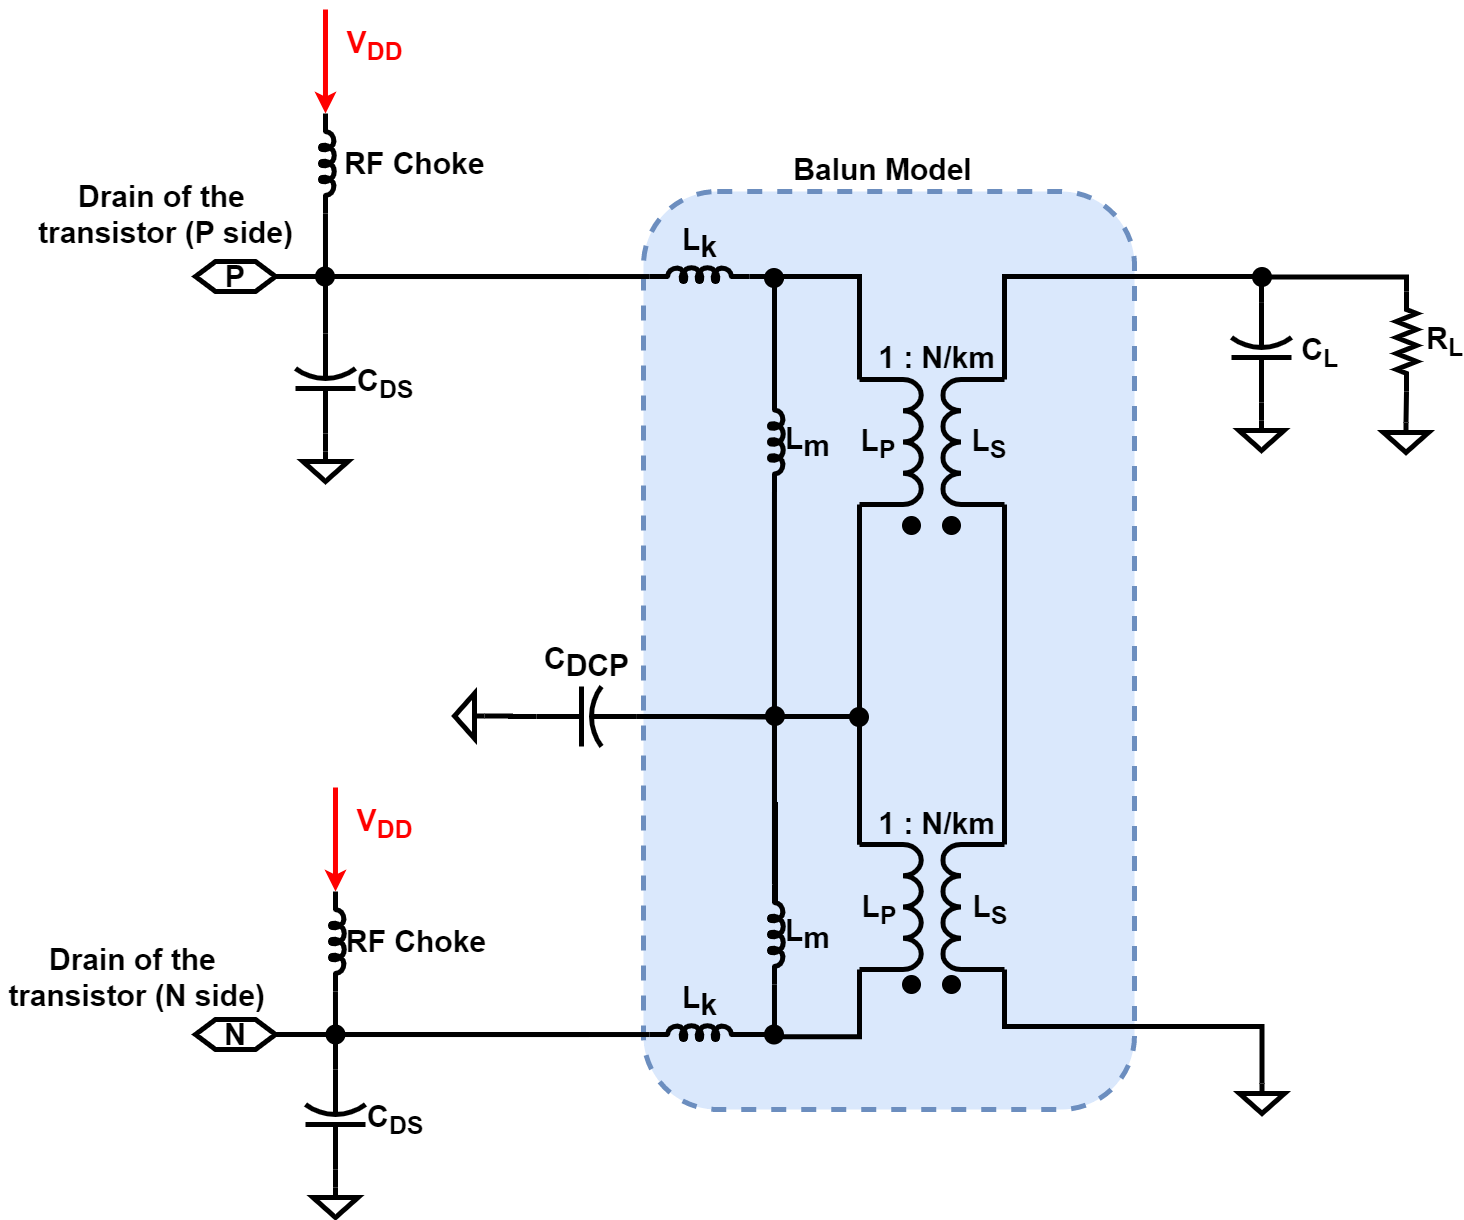
\includegraphics[width=1\textwidth]{Images/Design/Design_D_FC.png}
\caption{}
\label{fig:Design_D_FC}
\end{subfigure}
\caption{(a) Design B (Balun and $C_L$); (b) Design C (Balun, RF Choke, $L_2C_2$ \& $C_L$); (c) Design D (Balun, RF Choke \& $C_L$)}
\label{fig:Design_B_C_D}
\end{figure}

In this design (Figure \ref{fig:Design_B_FC}), $L_2C_2$ is removed so it reduces the number of unknowns. Like the previous case, differential mode analysis yields \textit{4} equations and there are \textit{4} unknowns, thus leading to a single set of values for $km =$ \textit{0.72}, $N =$ \textit{0.9}, $L_P =$ \textit{0.63 nH}, $C_L =$ \textit{3.96 pF}, unlike design A. $C_{DCP}$ is tuned to provide a short at $2\omega_0$ such that $C_{DCP}$ resonates with $L_P$, $L_{BND}$ and $C_{DS}$ which is obtained from the common mode analysis. Moreover, $C_{DCP}$ provides RF ground and blocks DC.

\subsection{Design C (with RF choke \& with $L_2C_2$)}
In this design (Figure \ref{fig:Design_C_FC}), $V_{DD}$ is supplied through RF choke unlike the previous designs. RF chokes are assumed to have a fixed value of \textit{5 nH}. The differential mode analysis yields \textit{4} equations similar to design A. Assuming $km =$ \textit{0.8}, the other unknowns are calculated as $N =$ \textit{1.14}, $L_P =$ \textit{2.23 nH}, $C_L =$ \textit{1.10 pF}, $C_2 =$ \textit{1.37 pF}.
Like design A, $C_2$ should resonate out with $L_2$ to get short at $2\omega_0$. Thus, $L_2 =$ \textit{0.8 nH}. 

\subsection{Design D (with RF choke \& no $L_2C_2$)}
 Unlike design C, $L_2C_2$ is removed in this design (Figure \ref{fig:Design_D_FC}). Also, RF choke should be calculated assuming $C_{DS}$ resonates with it at $\omega_0$ (RF Choke = \textit{2.35 nH}).
The differential mode analysis yields \textit{4} equations and the \textit{4} unknowns ($N =$ \textit{0.84}, $L_P =$ \textit{0.86 nH}, $C_L =$ \textit{3.95 pF}, $km =$ \textit{0.77}) can be calculated.
$C_{DCP}$ can be tuned to provide a short at $2\omega_0$.

\section{Results}
\label{section:Results}

Figures \ref{fig:Comp_1H} and \ref{fig:Comp_2H_imag}  show that all the \textit{4} designs satisfying the main CCF requirements which is decreasing trend of the reactive part at fundamental and increasing trend of the reactive part at $2^{nd}$ harmonic.
From Figure \ref{fig:Comp_1H}, it is seen that the real part at fundamental is flatter in the bandwidth \textit{2.1 - 2.7 GHz} for design A and C which, in turn, leads to constant $P_{OUT}$ in the specified bandwidth unlike design B and D. The $L_2C_2$ which acts as a varying capacitor at fundamental hold the reason for this. The designs B and D have a higher reactive part at the fundamental as compared to other designs which in turn leads to larger $\gamma$ value (refer equation \ref{eqn_CCF_imp}) and thus, higher peak factor (refer Figure \ref{fig:CCF_wave_VI}). Figures \ref{fig:Comp_2H_imag} and \ref{fig:Comp_3H_Mag} show that all the \textit{4} designs have similar response at $2^{nd}$ and $3^{rd}$ harmonic. 
%The impedance at \textit{2.1 GHz} and \textit{2.7 GHz} is less than \textit{200} $\Omega$ for all the \textit{4} designs.

\begin{figure}[!t]
\captionsetup{font=footnotesize}
\centering
\begin{subfigure}{0.5\textwidth}
\centering
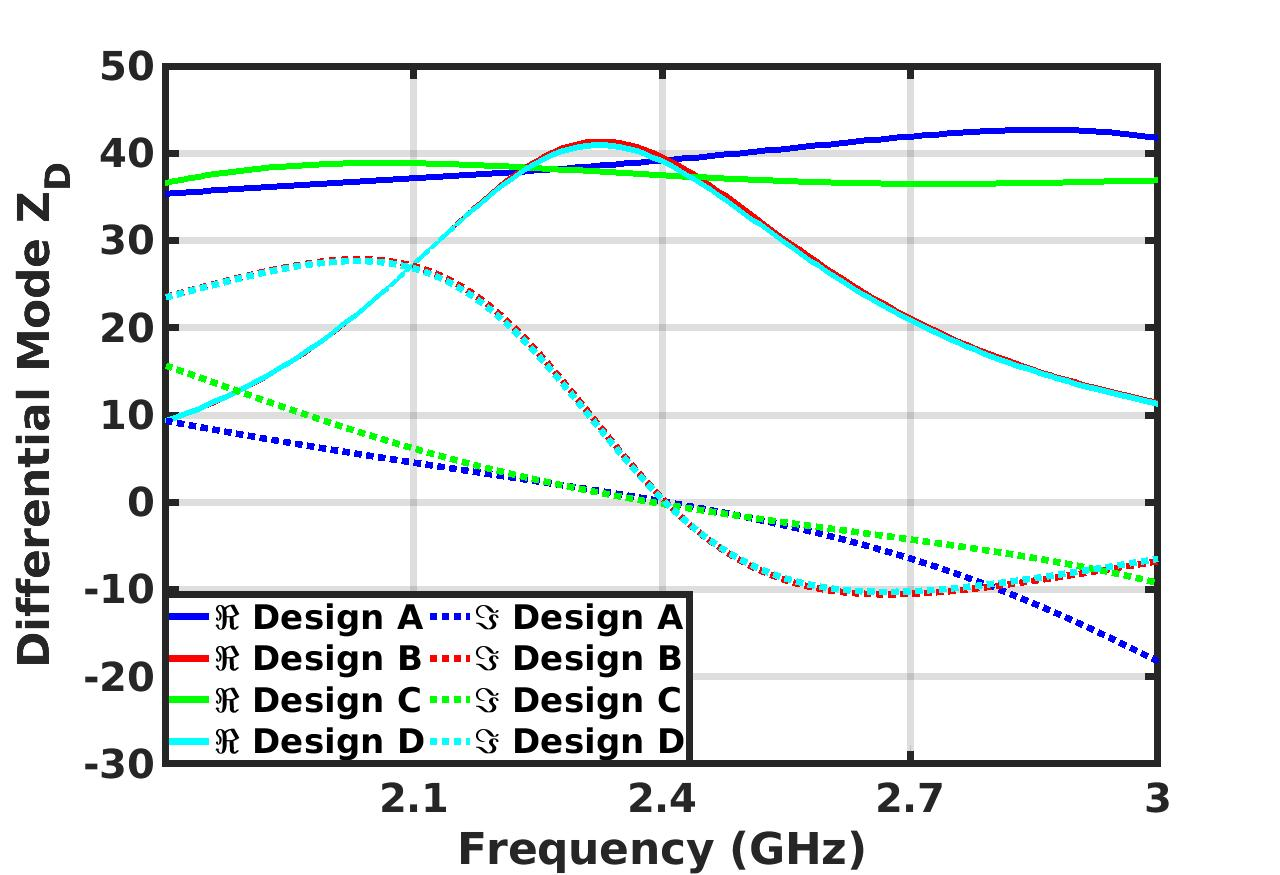
\includegraphics[width=0.65\textwidth]{Images/Output_Network_Comp/Comp_1H.jpg}
\caption{}
\label{fig:Comp_1H}
\end{subfigure}
\begin{subfigure}{0.24\textwidth}
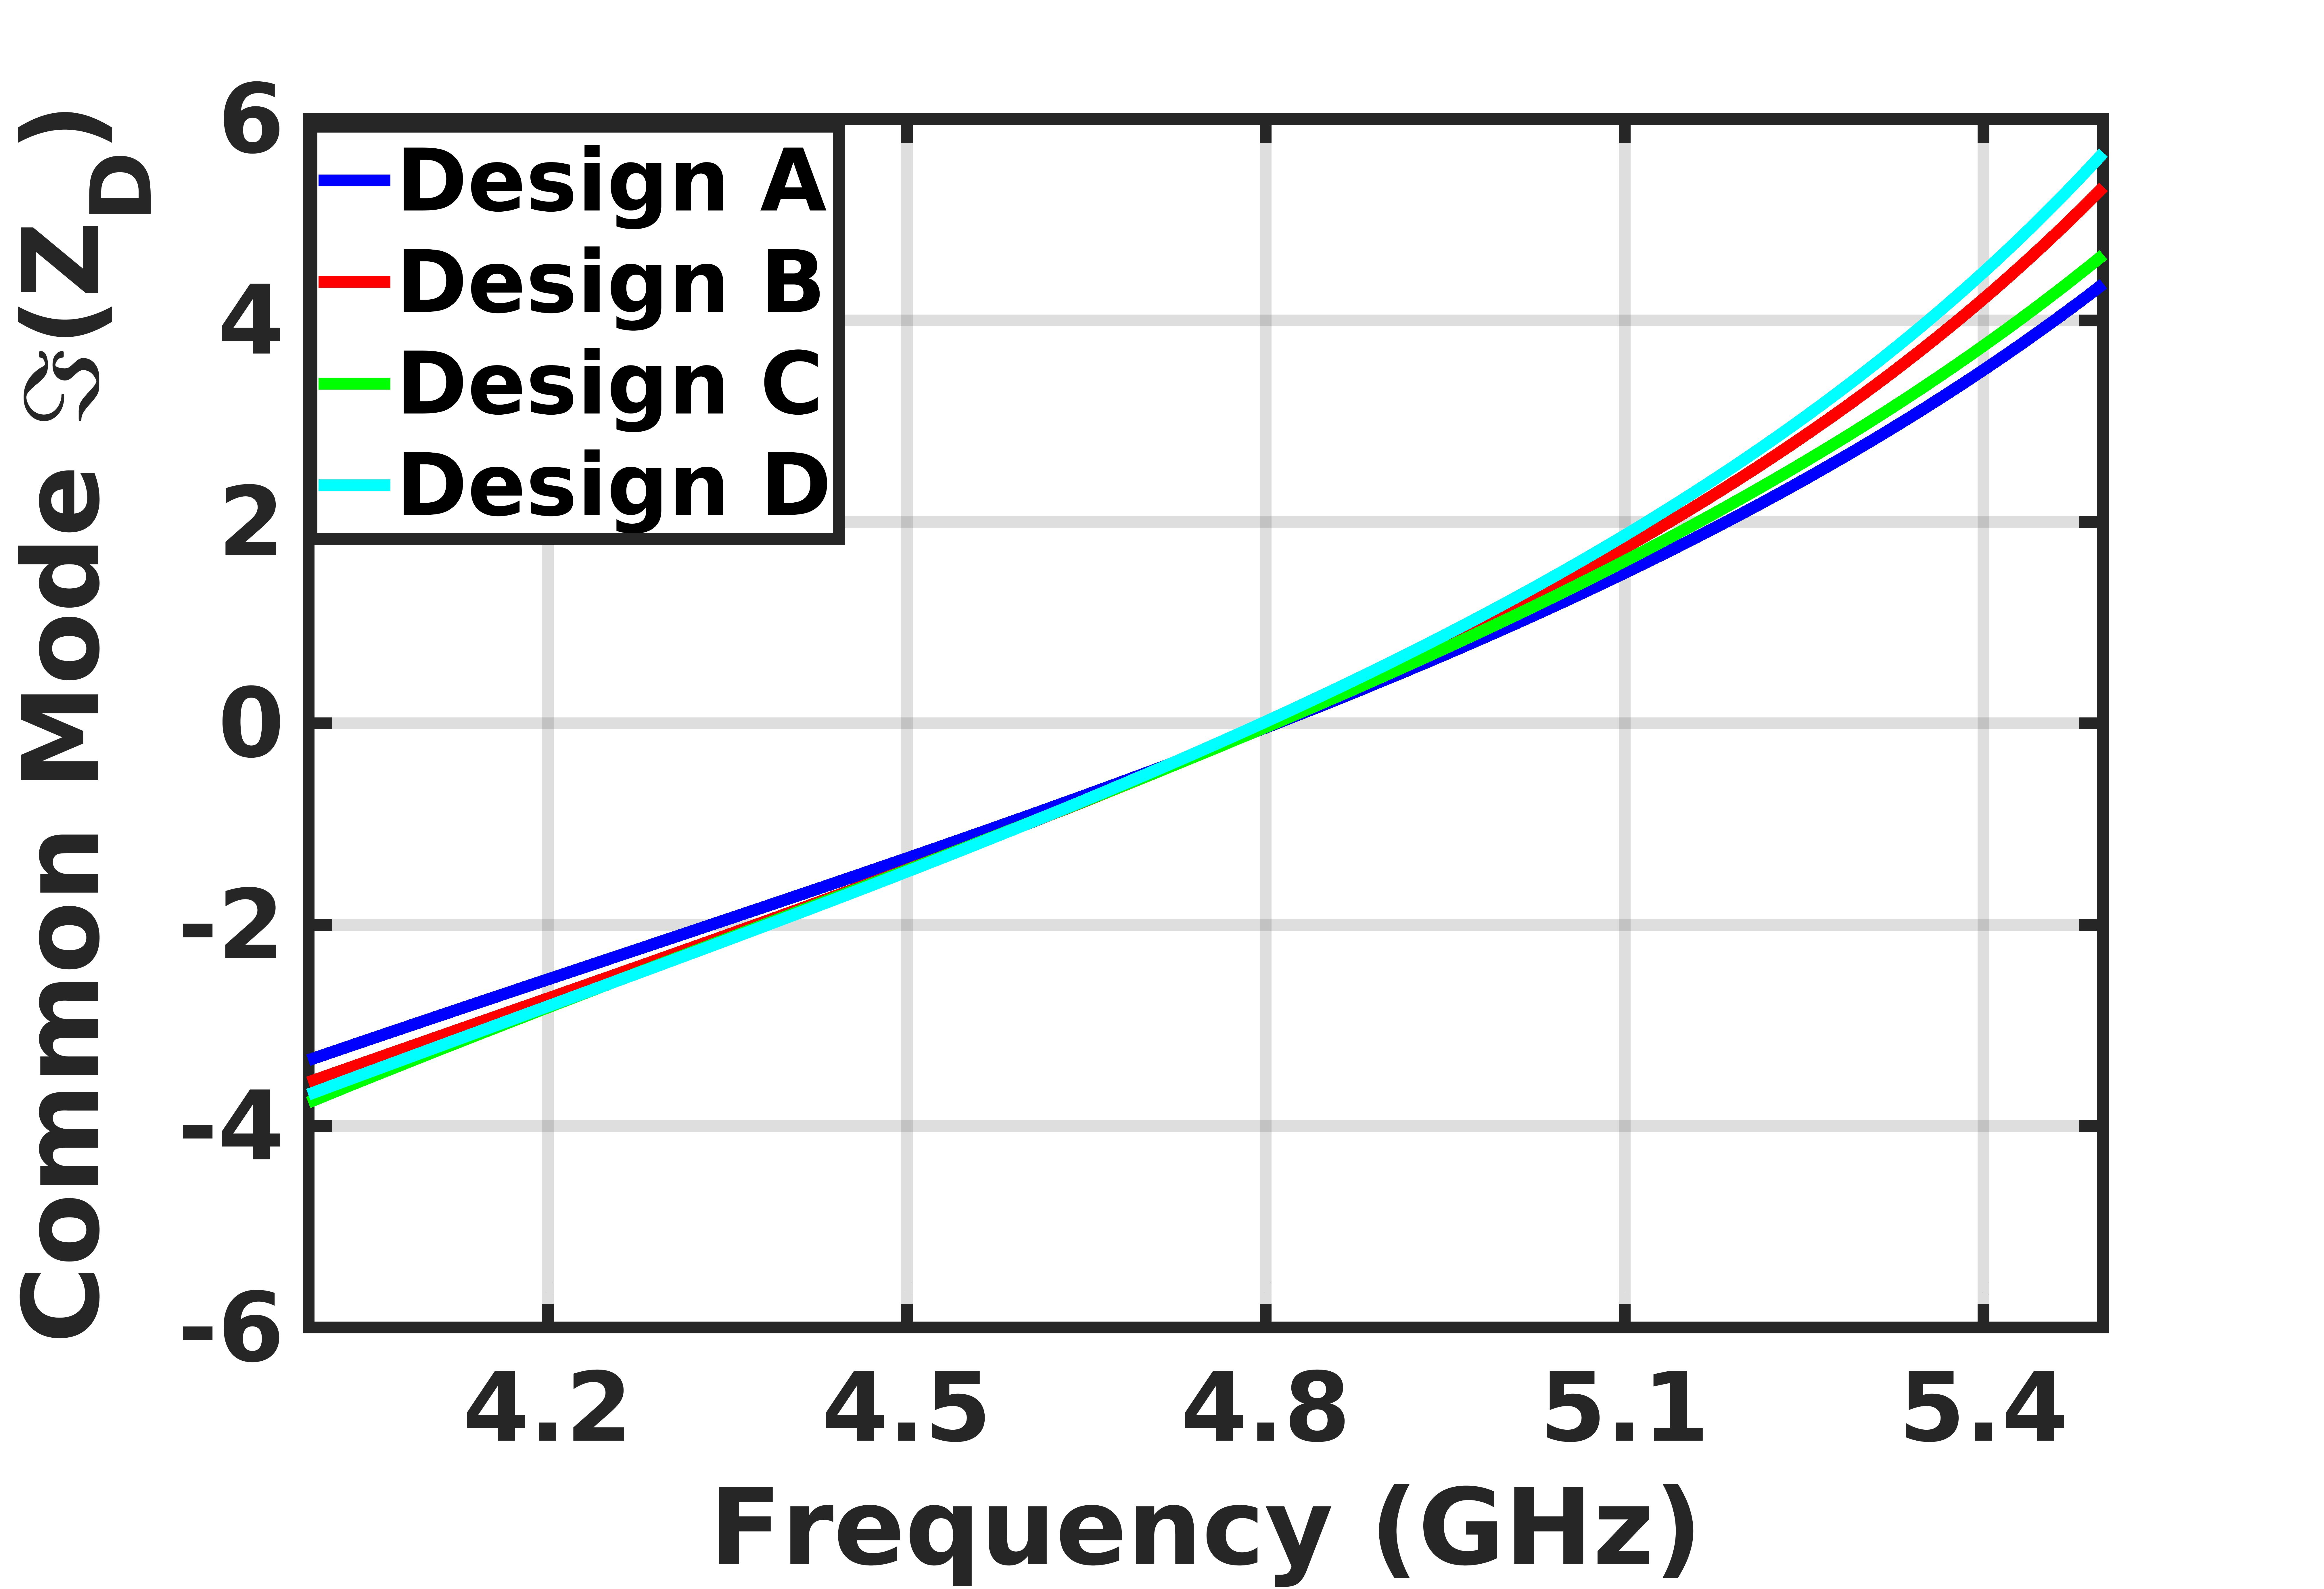
\includegraphics[width=1\textwidth]{Images/Output_Network_Comp/Comp_2H_imag.jpg}
\caption{}
\label{fig:Comp_2H_imag}
\end{subfigure}
\begin{subfigure}{0.24\textwidth}
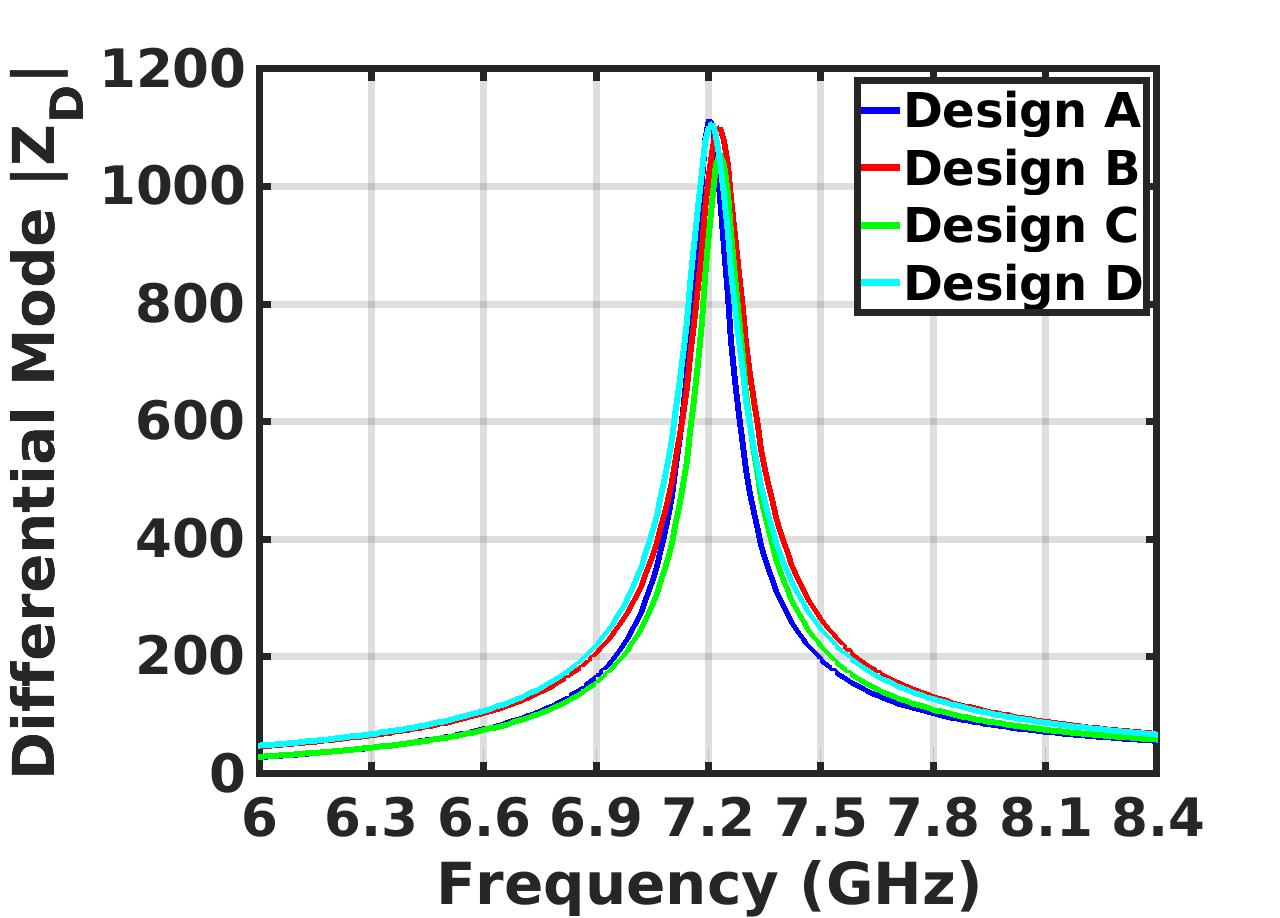
\includegraphics[width=1\textwidth]{Images/Output_Network_Comp/Comp_3H_Mag.jpg}
\caption{}
\label{fig:Comp_3H_Mag}
\end{subfigure}
\caption{(a) Impedance ($Z_D$) at $1^{st}$ harmonic; (b) Reactive part of $Z_D$ ($\Im(Z_D)$) at $2^{nd}$ harmonic; (c) Magnitude of $Z_D$ ($|Z_D|$) at $3^{rd}$ harmonic}
\label{fig:Comp_1H_2H_3H}
\vspace{-0.1in}
\end{figure}


The \textit{4} output networks are tested with an ideal output stage (single transistor which acts as a current source when turned on) in ADS. Figure \ref{fig:Comp_Pout_DE} shows there is a large variation in peak $P_{OUT}$ and maximum $\eta_D$ across the operational bandwidth for the design B and D, unlike design A and C. This variation can be attributed to the varying real part at the fundamental in those designs.
So from the simulation, it is seen that design A outperforms other designs since it has the least number of components as well as more constant $P_{\text{OUT}}$ and $\eta_D$ in the specified bandwidth.

\begin{figure}[!t]
\captionsetup{font=footnotesize}
\centering
\begin{subfigure}{0.24\textwidth}
\centering
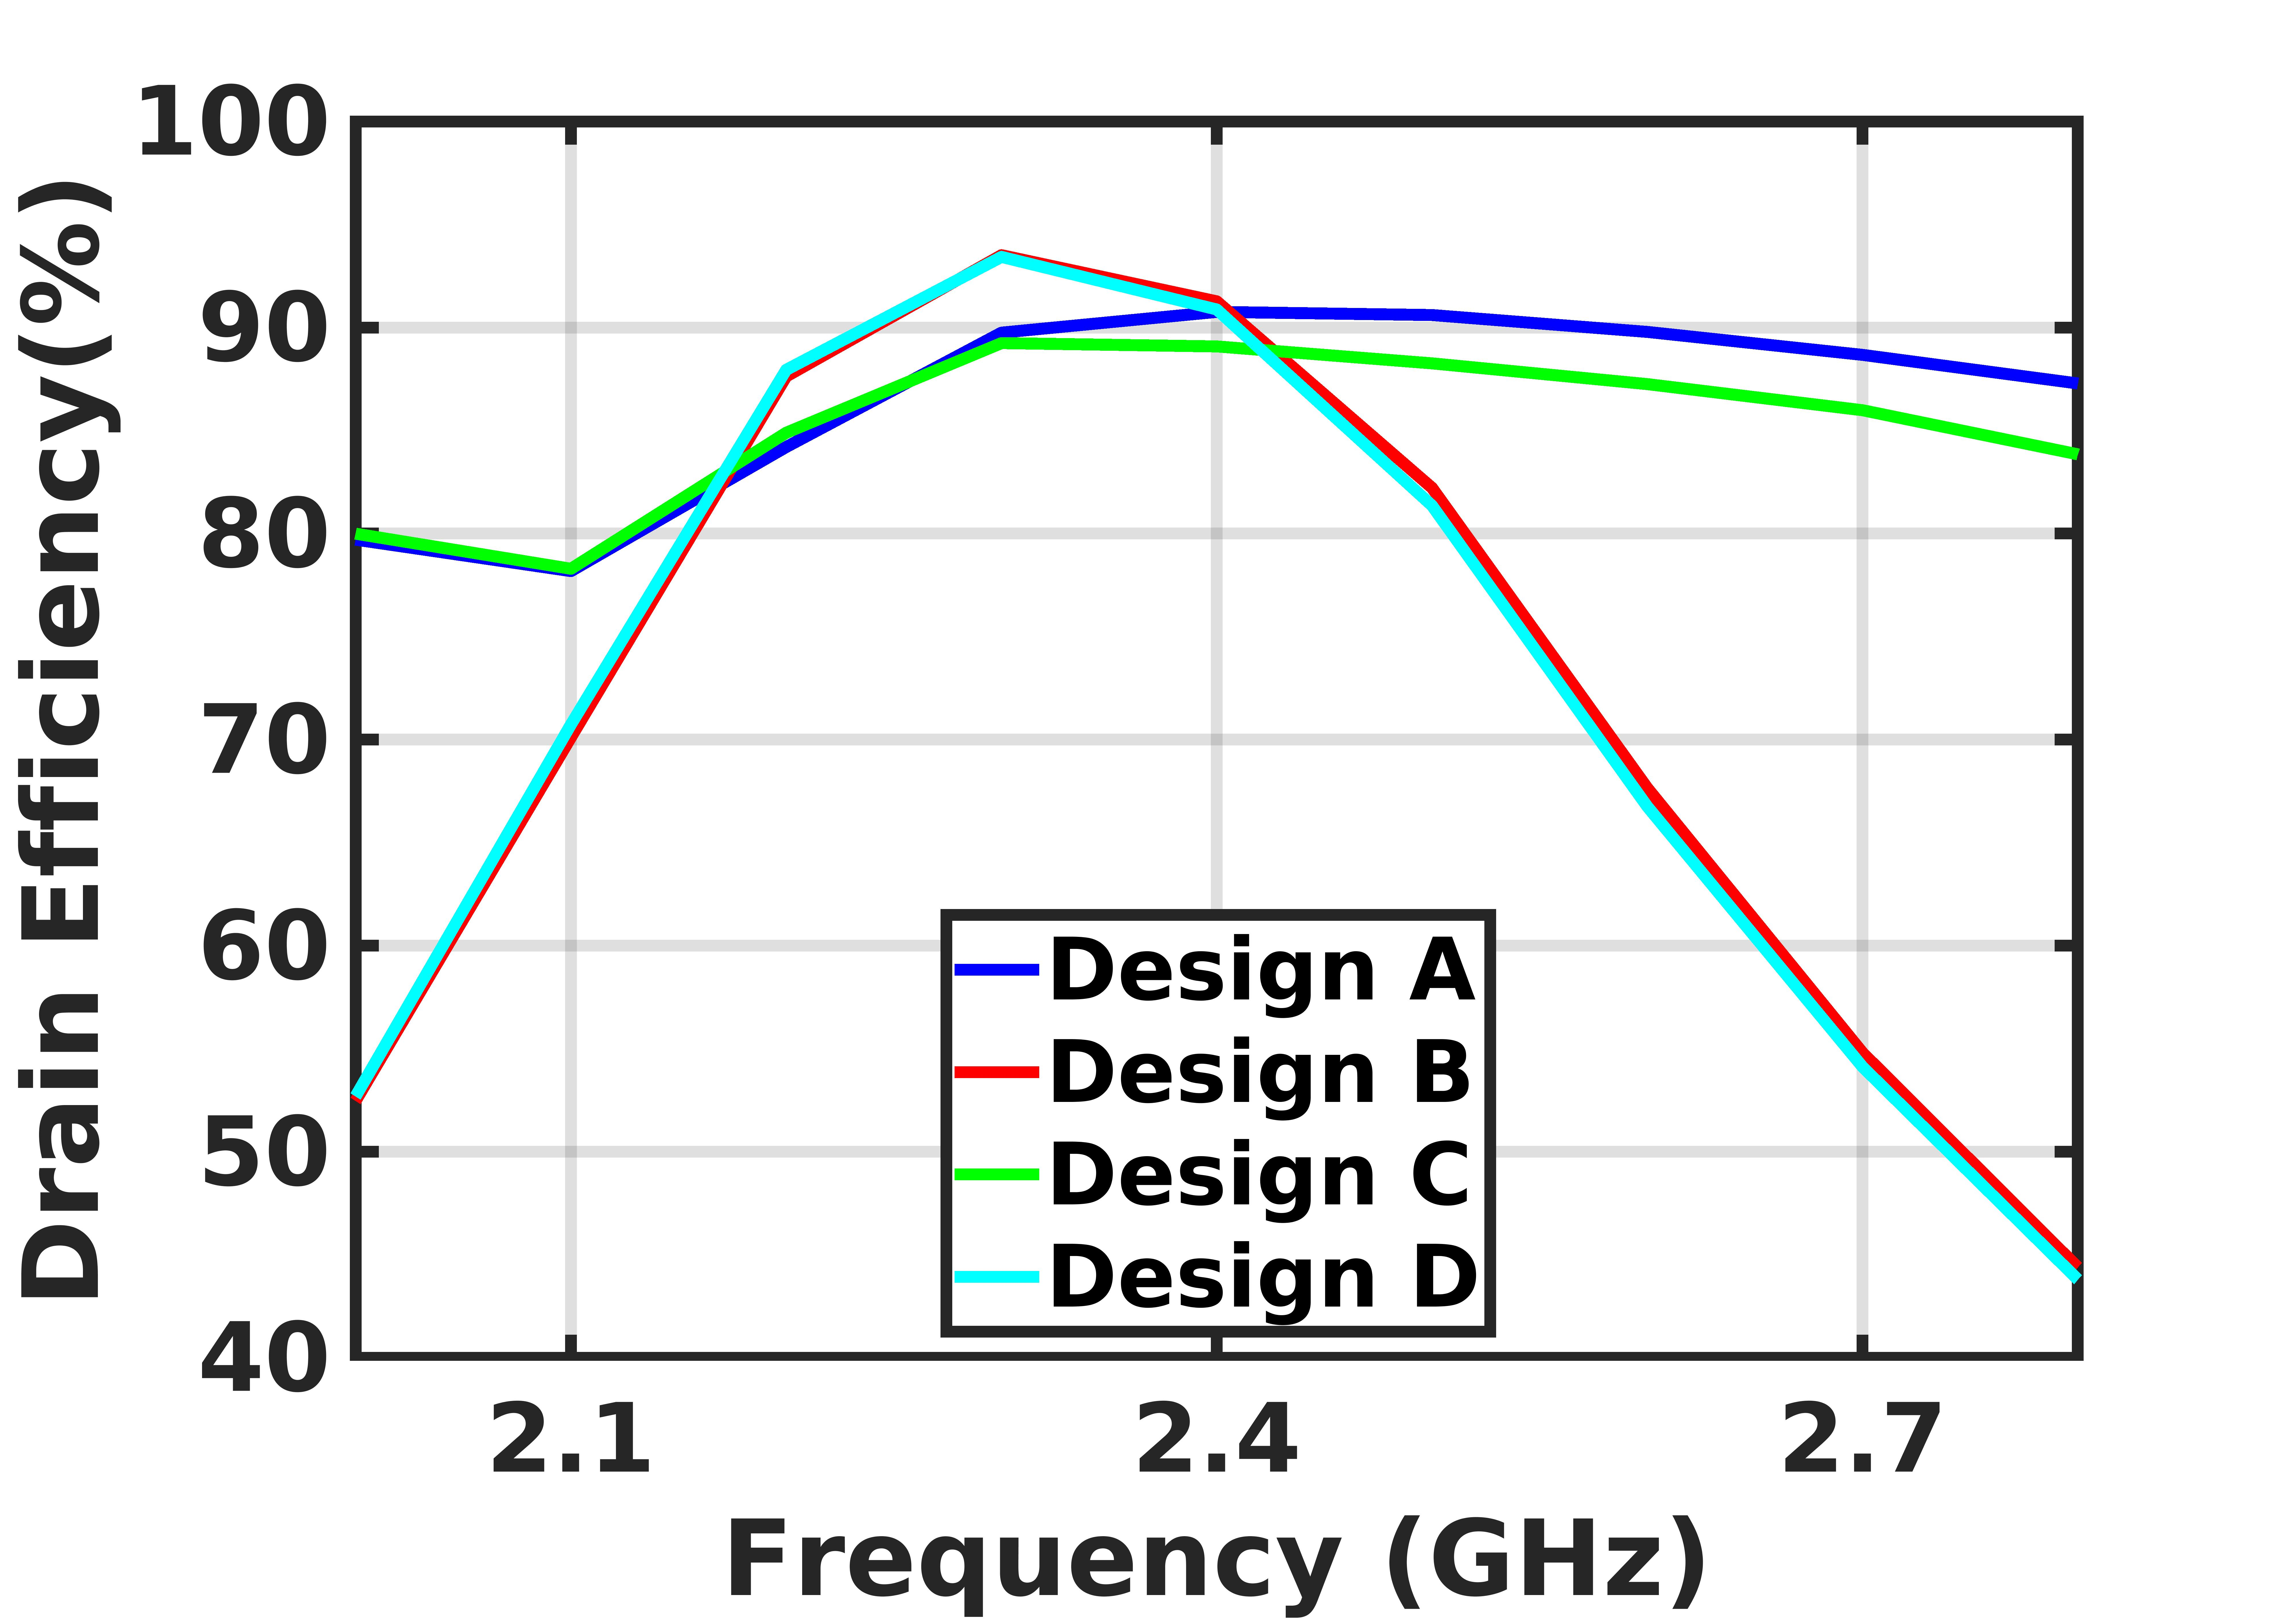
\includegraphics[width=1\textwidth]{Images/Output_Network_Comp/Comp_DE.jpg}
\caption{}
\label{fig:Comp_DE}
\end{subfigure}
\begin{subfigure}{0.24\textwidth}
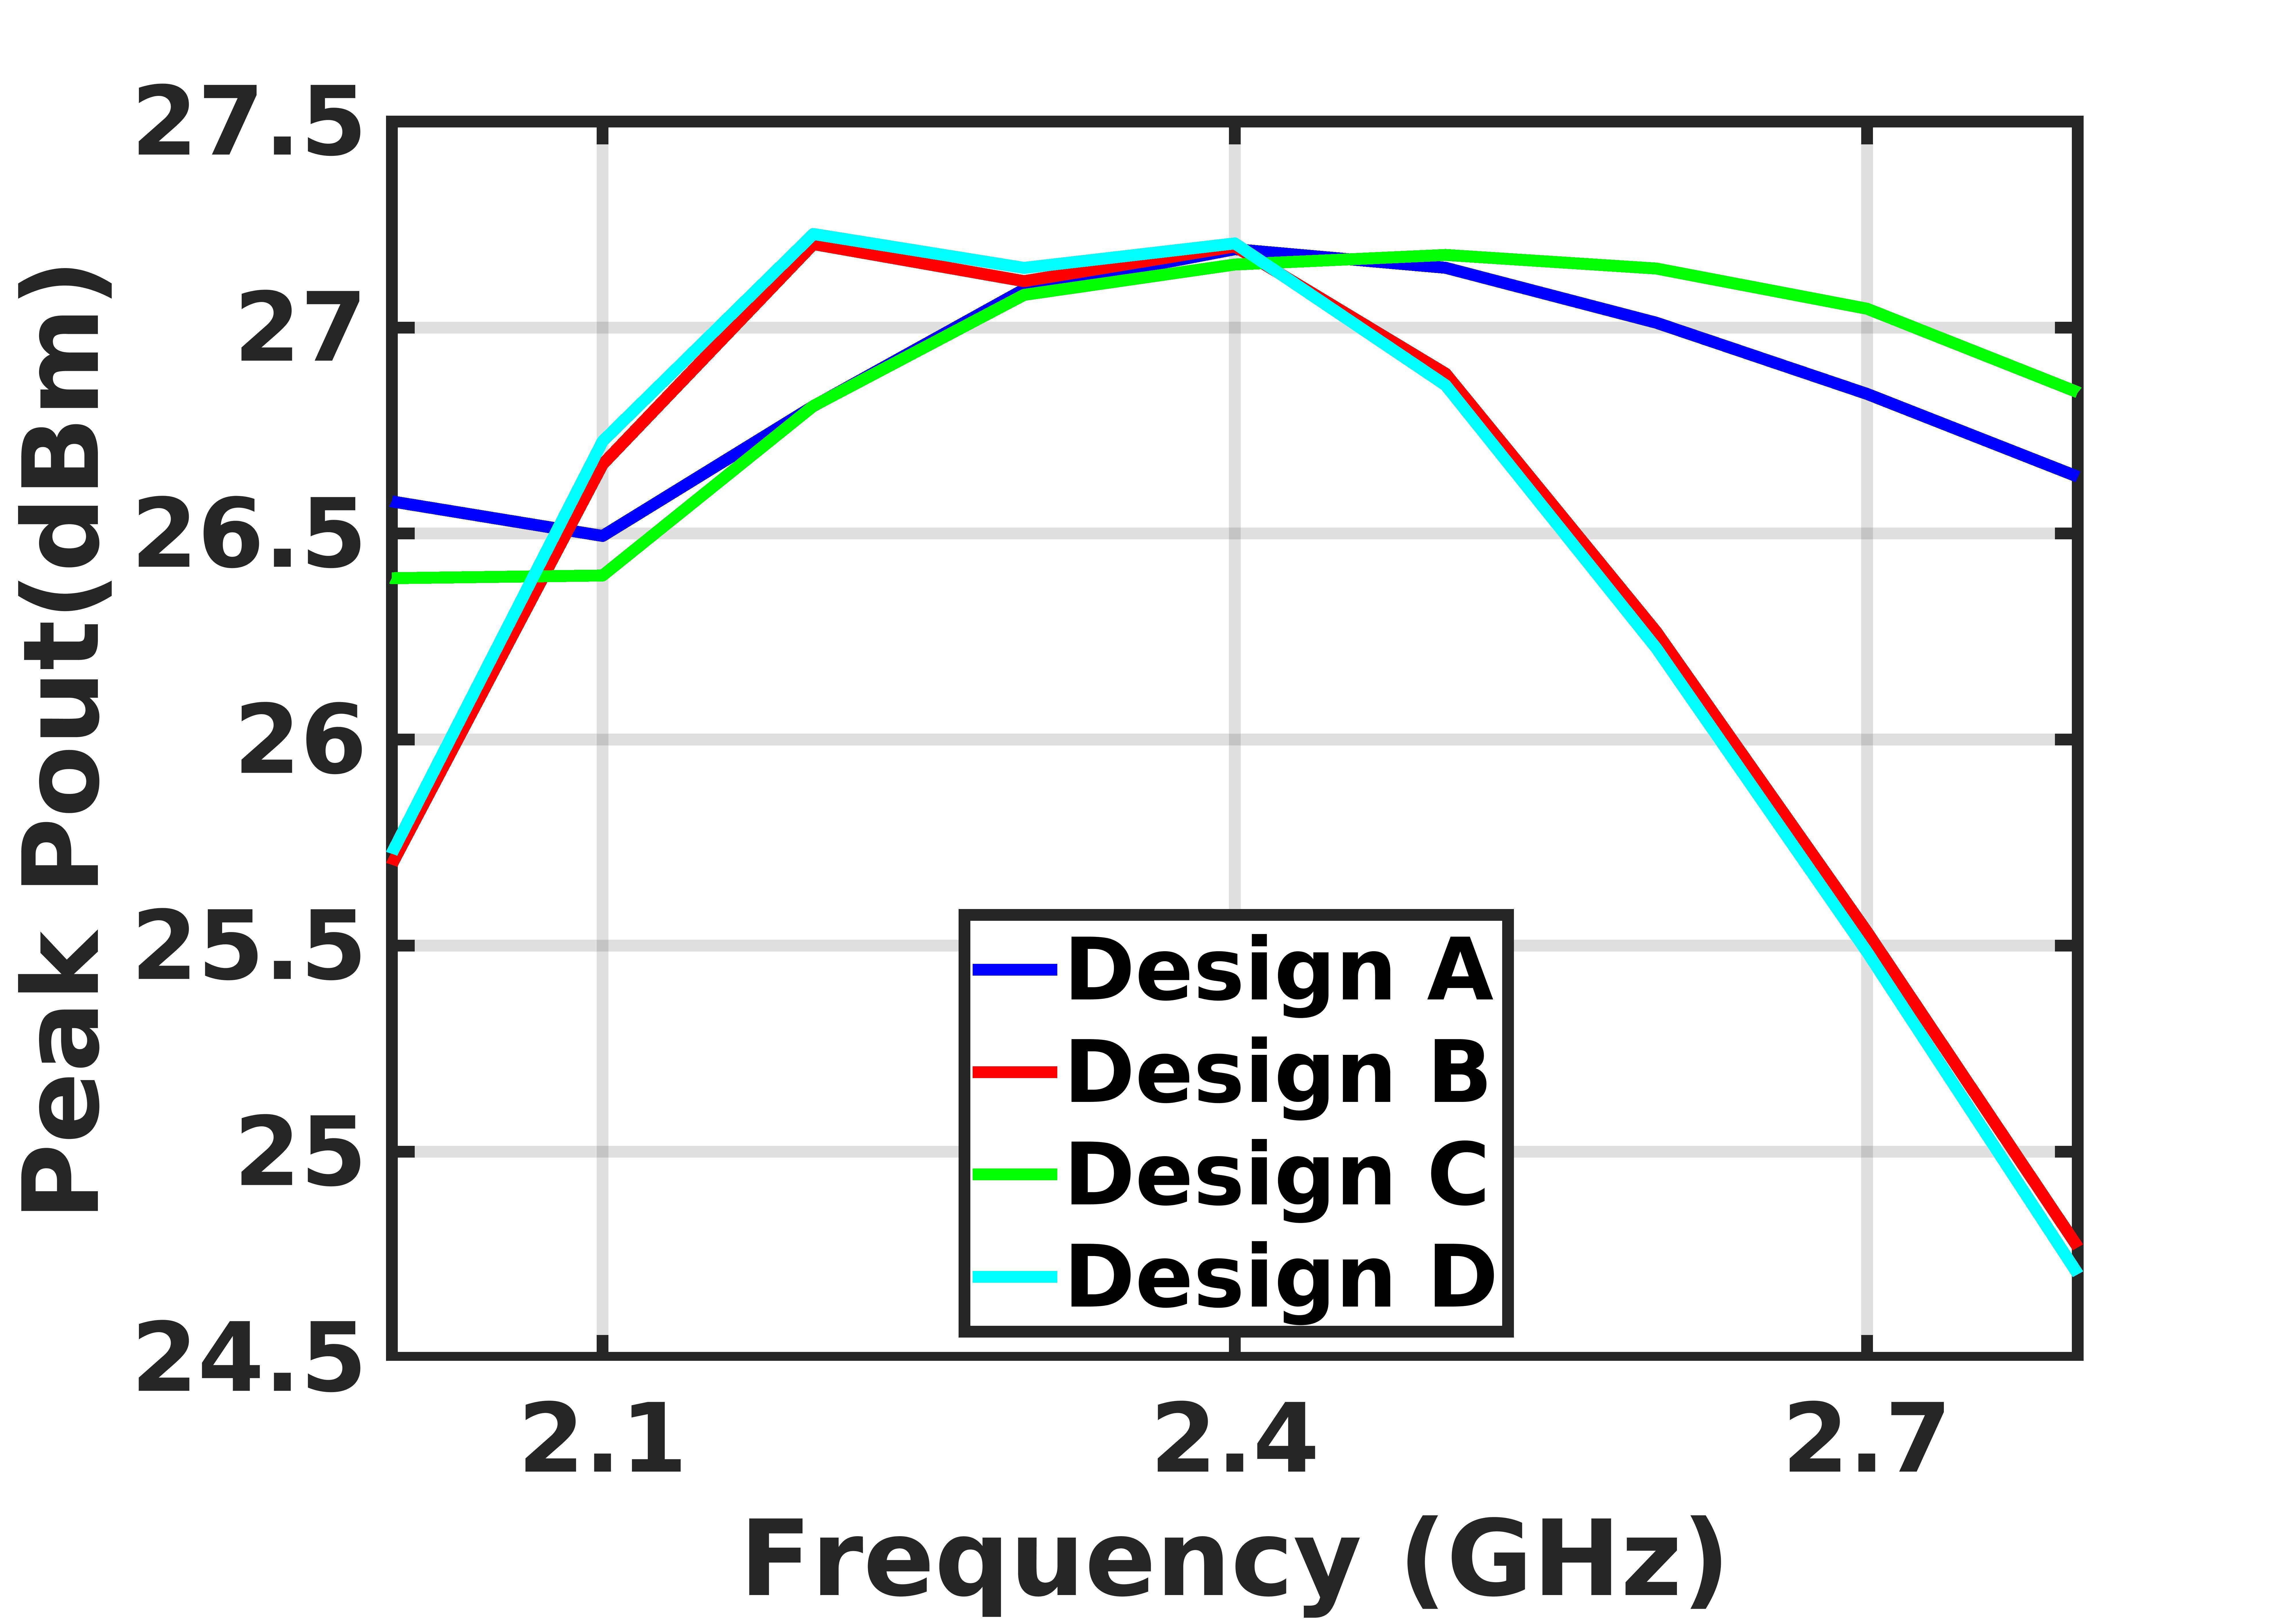
\includegraphics[width=1\textwidth]{Images/Output_Network_Comp/Comp_Pout.jpg}
\caption{}
\label{fig:Comp_Pout}
\end{subfigure}
\caption{(a) Maximum drain efficiency across frequency for 4 different output network; (b) Peak $P_{OUT}$ across frequency for 4 different output network;}
\label{fig:Comp_Pout_DE}
\vspace{-0.25in}
\end{figure}

\section{Conclusion}
\label{section:Conclusion}
This paper presented CCF's \color{blue} wide operational bandwidth advantage over its class F companion. It detailed the primary requirement of the CCF PA output network, which is \color {black} if the reactive part of $1^{st}$ harmonic decreases, then the reactive part of $2^{nd}$ harmonic should increase. \color{blue} Furthermore, \color{black} the procedure to design the \textit{\color{blue} four \color{black}}different output networks for the \color{blue}\textit{2.1 -- 2.7 GHz} band was \color{black} \color{blue} proposed and analyzed in detail. \color{black} Consequently, \color{black}design A\color {blue}, \color{black} with no RF choke and \color{blue} including a 2$^{nd}$ harmonic trap\color{black} \color {blue}, \color{black}  was chosen because it \color{blue} offers relatively \color{black} constant \color{blue} output RF power \color{black} in the \color{blue} desired frequency band \color{black} with the least number of components.

\bibliographystyle{IEEEtran}
\bibliography{disseration.bib}

\end{document}


